
% \documentclass[10pt,journal,cspaper,compsoc]{IEEEtran}
\documentclass[10pt,journal]{IEEEtran}

%
\ifCLASSOPTIONcompsoc
  % IEEE Computer Society needs nocompress option
  % requires cite.sty v4.0 or later (November 2003)
  % \usepackage[nocompress]{cite}
\else
  % normal IEEE
  % \usepackage{cite}
\fi

% *** GRAPHICS RELATED PACKAGES ***
%
\ifCLASSINFOpdf
  % \usepackage[pdftex]{graphicx}
  % declare the path(s) where your graphic files are
  % \graphicspath{{../pdf/}{../jpeg/}}
  % and their extensions so you won't have to specify these with
  % every instance of \includegraphics
  % \DeclareGraphicsExtensions{.pdf,.jpeg,.png}
\else
  % or other class option (dvipsone, dvipdf, if not using dvips). graphicx
  % will default to the driver specified in the system graphics.cfg if no
  % driver is specified.
  % \usepackage[dvips]{graphicx}
  % declare the path(s) where your graphic files are
  % \graphicspath{{../eps/}}
  % and their extensions so you won't have to specify these with
  % every instance of \includegraphics
  % \DeclareGraphicsExtensions{.eps}
\fi
% graphicx was written by David Carlisle and Sebastian Rahtz. It is
% required if you want graphics, photos, etc. graphicx.sty is already
% installed on most LaTeX systems. The latest version and documentation can
% be obtained at:
% http://www.ctan.org/tex-archive/macros/latex/required/graphics/
% Another good source of documentation is "Using Imported Graphics in
% LaTeX2e" by Keith Reckdahl which can be found as epslatex.ps or
% epslatex.pdf at: http://www.ctan.org/tex-archive/info/
%
% latex, and pdflatex in dvi mode, support graphics in encapsulated
% postscript (.eps) format. pdflatex in pdf mode supports graphics
% in .pdf, .jpeg, .png and .mps (metapost) formats. Users should ensure
% that all non-photo figures use a vector format (.eps, .pdf, .mps) and
% not a bitmapped formats (.jpeg, .png). IEEE frowns on bitmapped formats
% which can result in "jaggedy"/blurry rendering of lines and letters as
% well as large increases in file sizes.
%
% You can find documentation about the pdfTeX application at:
% http://www.tug.org/applications/pdftex



% correct bad hyphenation here
\hyphenation{op-tical net-works semi-conduc-tor}

\usepackage{listings}
\usepackage[table]{xcolor}
\usepackage{graphicx}
\usepackage{amsmath}
\usepackage{amssymb}
\usepackage{color}
\usepackage{epsfig}
\usepackage{tabularx}
\usepackage{ctable}
\usepackage{multirow}
\usepackage{subfigure}
\usepackage{mathrsfs}
\usepackage{mathtools}
\usepackage{hyperref}
\usepackage{pbox}

\newcommand{\Songfan}[1]{\textcolor{red}{#1}}

\newcommand{\argmin}{\arg\!\min}
\newcommand{\argmax}{\arg\!\max}

\begin{document}
%
% paper title
% can use linebreaks \\ within to get better formatting as desired
\title{A Dense Flow-based Framework for Real-time Streaming Object Registration in Compound Motion}
%Understanding Consumer Preference for Advertisement\\from Facial Expression}
%
%
% author names and IEEE memberships
% note positions of commas and nonbreaking spaces ( ~ ) LaTeX will not break
% a structure at a ~ so this keeps an author's name from being broken across
% two lines.
% use \thanks{} to gain access to the first footnote area
% a separate \thanks must be used for each paragraph as LaTeX2e's \thanks
% was not built to handle multiple paragraphs
%
%
%\IEEEcompsocitemizethanks is a special \thanks that produces the bulleted
% lists the Computer Society journals use for "first footnote" author
% affiliations. Use \IEEEcompsocthanksitem which works much like \item
% for each affiliation group. When not in compsoc mode,
% \IEEEcompsocitemizethanks becomes like \thanks and
% \IEEEcompsocthanksitem becomes a line break with idention. This
% facilitates dual compilation, although admittedly the differences in the
% desired content of \author between the different types of papers makes a
% one-size-fits-all approach a daunting prospect. For instance, compsoc
% journal papers have the author affiliations above the "Manuscript
% received ..."  text while in non-compsoc journals this is reversed. Sigh.

\author{Songfan~Yang,~\IEEEmembership{Member,~IEEE,}
				Le~An,
				Mingyang~Li,~\IEEEmembership{Student Member,~IEEE,}
        Ninad~Thakoor,~\IEEEmembership{Member,~IEEE,}
        and~Bir~Bhanu,~\IEEEmembership{Fellow,~IEEE}% <-this % stops a space
\IEEEcompsocitemizethanks{\IEEEcompsocthanksitem Acknowledgment: \IEEEcompsocthanksitem \protect\\ S.~Yang is with the College of Electronics and Information Engineering at Sichuan University, Chengdu, China 610064. E-mail: syang@scu.edu.cn \protect\\
L.~An is with BRIC, University of North Carolina at Chapel Hill, Chapel
Hill, NC 27599 USA. E-mail: lan004@unc.edu \protect\\
M.~Li is with University of California, Riverside, CA 92521 USA. Email: mingyangli009@gmail.com \protect\\
N.~Thakoor,~and~B.~Bhanu are with the Center for Research in Intelligent Systems, University of California, Riverside, CA 92521 USA.\protect\\
E-mail: \{nthakoor,~bhanu\}@ee.ucr.edu}% <-this % stops a space
\thanks{}}

% note the % following the last \IEEEmembership and also \thanks -
% these prevent an unwanted space from occurring between the last author name
% and the end of the author line. i.e., if you had this:
%
% \author{....lastname \thanks{...} \thanks{...} }
%                     ^------------^------------^----Do not want these spaces!
%
% a space would be appended to the last name and could cause every name on that
% line to be shifted left slightly. This is one of those "LaTeX things". For
% instance, "\textbf{A} \textbf{B}" will typeset as "A B" not "AB". To get
% "AB" then you have to do: "\textbf{A}\textbf{B}"
% \thanks is no different in this regard, so shield the last } of each \thanks
% that ends a line with a % and do not let a space in before the next \thanks.
% Spaces after \IEEEmembership other than the last one are OK (and needed) as
% you are supposed to have spaces between the names. For what it is worth,
% this is a minor point as most people would not even notice if the said evil
% space somehow managed to creep in.



% The paper headers
\markboth{IEEE Transactions on Image Processing}%
{Shell \MakeLowercase{\textit{et al.}}: Bare Demo of
IEEEtran.cls for Computer Society Journals}
% The only time the second header will appear is for the odd numbered pages
% after the title page when using the twoside option.
%
% *** Note that you probably will NOT want to include the author's ***
% *** name in the headers of peer review papers.                   ***
% You can use \ifCLASSOPTIONpeerreview for conditional compilation here if
% you desire.


% for Computer Society papers, we must declare the abstract and index terms
% PRIOR to the title within the \IEEEcompsoctitleabstractindextext IEEEtran
% command as these need to go into the title area created by \maketitle.
\IEEEcompsoctitleabstractindextext{%
\begin{abstract}

\Songfan{A moving object often has elastic and deformable surfaces (e.g., the human head). Tracking and measuring surface deformation while the object body itself also moves via video analysis is a challenging problem with many applications.  For example, video-based facial expression recognition requires to track non-rigid motions of facial features without being affected by any rigid motion of the head. In this paper, we present a video alignment framework to extract and characterize surface deformations with respect to a fixed reference (a canonical form) accompanied by rigid-body motions.} We define a general model for object alignment in a Baysian framework, and rigorously show that a special case of the model results in a SIFT-flow- and optical-flow-based least-square problem. We demonstrate that dynamic programming can be used to speed up the computation. The proposed algorithm has a wide range of applications, including the analysis of subtle facial muscle dynamics in spontaneous expressions, vehicle recognition, and image super-resolution.  Experimental and quantitative results demonstrate the efficacy of the proposed algorithm.


\end{abstract}
% IEEEtran.cls defaults to using nonbold math in the Abstract.
% This preserves the distinction between vectors and scalars. However,
% if the journal you are submitting to favors bold math in the abstract,
% then you can use LaTeX's standard command \boldmath at the very start
% of the abstract to achieve this. Many IEEE journals frown on math
% in the abstract anyway. In particular, the Computer Society does
% not want either math or citations to appear in the abstract.

% Note that keywords are not normally used for peer review papers.
\begin{keywords}
Object registration, spontaneous facial expression, SIFT flow, optical flow, super-resolution
\end{keywords}}


% make the title area
\maketitle


% To allow for easy dual compilation without having to reenter the
% abstract/keywords data, the \IEEEcompsoctitleabstractindextext text will
% not be used in maketitle, but will appear (i.e., to be "transported")
% here as \IEEEdisplaynotcompsoctitleabstractindextext when compsoc mode
% is not selected <OR> if conference mode is selected - because compsoc
% conference papers position the abstract like regular (non-compsoc)
% papers do!
\IEEEdisplaynotcompsoctitleabstractindextext
% \IEEEdisplaynotcompsoctitleabstractindextext has no effect when using
% compsoc under a non-conference mode.


% For peer review papers, you can put extra information on the cover
% page as needed:
% \ifCLASSOPTIONpeerreview
% \begin{center} \bfseries EDICS Category: 3-BBND \end{center}
% \fi
%
% For peerreview papers, this IEEEtran command inserts a page break and
% creates the second title. It will be ignored for other modes.
\IEEEpeerreviewmaketitle


\section{Introduction}

\IEEEPARstart{V}{ideo} registration is an important problem for video processing, computer vision and pattern recognition. It has various applications such as face recognition~\cite{Wagner2009}, facial expression recognition~\cite{Valstar12}, image stitching~\cite{Szeliski06}, color demosaicking \cite{Wu_TIP06}, and etc. Depending upon different applications, there can be specific requirements for the registration techniques~\cite{Uenohara95}~\cite{Caspi_PAMI02}. \Songfan{Broadly speaking, in the process of registration most algorithms overlay objects spatially via motion estimation and compensation. 
}

\Songfan{Video registration becomes a more challenging problem if there are object surface deformations which are further compounded by rigid-body motions or/and camera motion; in particular, if subtle surface non-rigid motions have to be detected and precisely characterized in applications like medical imaging and facial expression. To appreciate the difficulties in precisely characterizing surface deformation amidst complex compound motion, let us examine a concrete example: the human facial expression analysis, in which the non-rigid muscle motion is of the central focus.  Accurate facial expression analysis is hampered by the following complications:} 

\begin{figure}[!t]
	\centering
		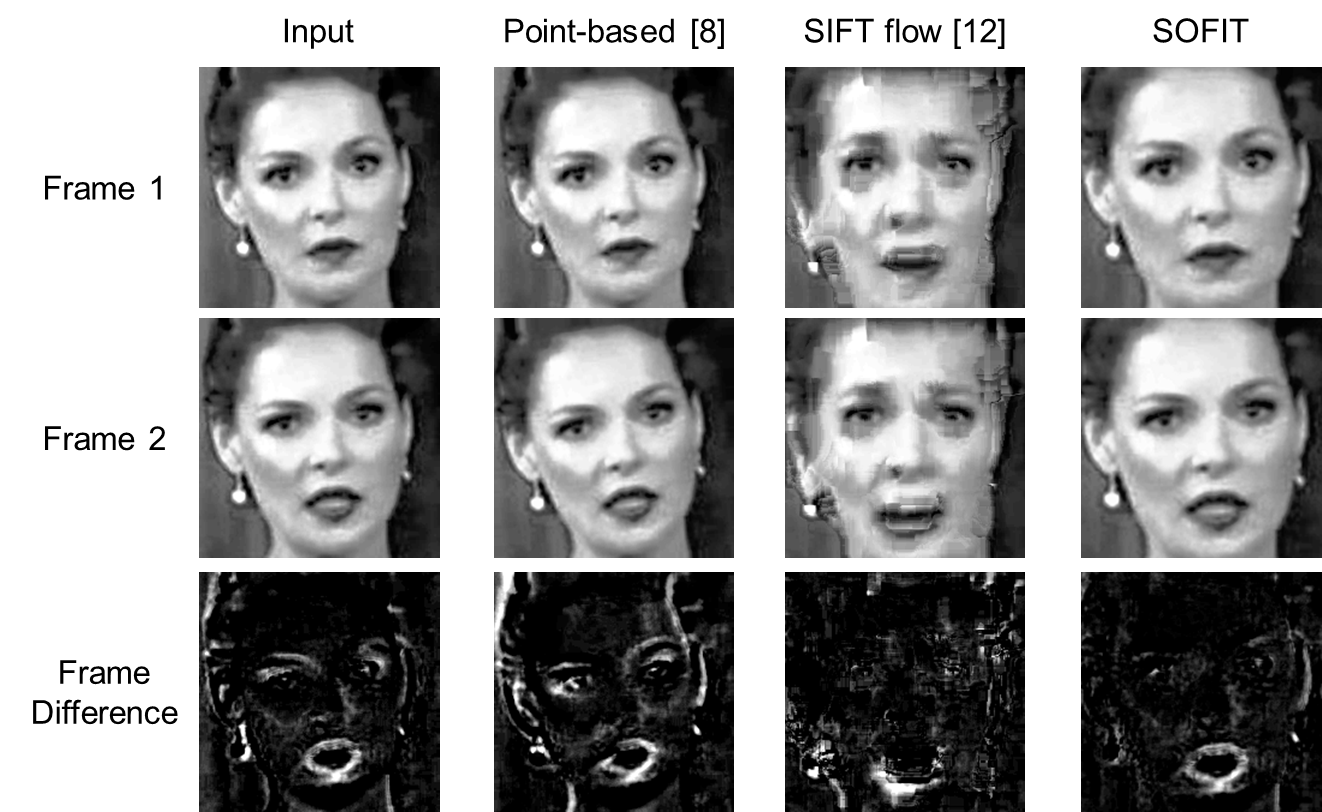
\includegraphics[width=\columnwidth]{fig/regComp.png}
	\caption{Comparison of registration results. Row 3 is the absolute difference of frame 1 and frame 2. Column 2 is the point-based affine registration method used in~\cite{Littlewort_CERT_FG2011}~\cite{Valstar_SMCB12}, where affine transformation is computed from 68 facial feature points generated by the state-of-the-art detector~\cite{Zhu_CVPR12}. Column 3 uses SIFT flow~\cite{Liu_PAMI11} to align with the Avatar Reference face model from~\cite{Yang_SMCB12}. Ideally, we would like the frame difference to show only at locations where the non-rigid motion is present (mouth area in this case). The proposed method, SOFIT, achieves the most plausible result.}
	\label{fig:regComp}
\end{figure}

\begin{enumerate}
\item The facial muscle motion is non-rigid. In the real data facial expressions are coupled with rigid motion of head pose.
\item The head pose comprises of both in-plane rotation and out-of-plane rotation.
\item The muscle motion is subtle in real-world spontaneous expressions.
\item The data are streaming instead of being in a batch form.
\item The consecutive frames should comply with temporal smoothness constraint for micro-expression analysis.
\item The imaging condition is varying, such as the illumination or resolution of the face region.
%\vspace{-5pt}
\end{enumerate}

In this paper, we propose a new video registration approach, termed SIFT and optical flow image transform (SOFIT)\footnote{supplementary materials available at the project page:~\url{http://ee.ucr.edu/~syang/sofit/index.html}}, that tackles the aforementioned challenges in \Songfan{aligning object features through video frames in the presence of compounded surface deformation and rigid motion.}

\Songfan{
For the purposes of recognition, super-resolution, video compression, etc., the deformed object should be performed with respect to a canonical form or reference model.
For instance, such a reference model is instrumental in facial expression analysis ~\cite{Yang_SMCB12}.
}

Facial muscle motion is similar for the same expression irrespective of the person~\cite{Ekman78}, but the facial feature location (such as eyes, nose, mouth) of different people varies. Thus, finding a canonical reference feature location for all the faces is favorable for analyzing the dynamics of facial features across population. \Songfan{In the proposed SOFIT approach, we need to transform every frame of the streaming video data into a canonical pose by neutralizing the effects of rigid body motion on the imaged deformable object.}

\Songfan{To further clarify the above design objective, let us examine, via Fig.~\ref{fig:regComp}, how different video registration methods behave when being applied to register frame 2 with respect to frame 1.  All methods in this figure are able to account for the in-plane head rotation. However, as illustrated by the frame difference images (row 3) for the point-based affine transformation (column 2) and the SIFT flow transformation (column 3), there is a motion on most parts of the face. This is similar to the original face image (column 1) where the image is the output of Viola-Jones face detector~\cite{Viola_IJCV04} and is not registered. This suggests us to impose the temporal smoothness constraint so that the frame difference is small for areas with no motion; while for areas with motion (mouth area in this case), the frame difference should capture this change, as demonstrated by the results of the proposed method (column 4).}

In this paper, we model the alignment-of-compound-motion problem by three parts. First, each frame is aligned with respect to a reference frame in a general distance measure. It is then instantiated to the SIFT flow criterion thereafter. Second, our model enforces a smoothness constraint on adjacent frames. It is realistic for the consecutive frames to comply with the smoothness constraint. We realize this by depending this current transformation estimation on a number of previous frames in an optical flow criterion. Third, large transformation is penalized to prevent over-fitting. 

\Songfan{
We also extend this approach to register many other classes of objects and demonstrate a range of applications in areas such as vehicle recognition and image super-resolution. 
}

The rest of the paper is organized as follows. After reviewing the related work and highlighting our contribution in Section~\ref{sec:relatedWork_Contribution}, Section~\ref{sec:approach} presents our general model as well as the solution to the registration problem using the dense flow approximation to estimate the affine transformation parameters. The experimental results and discussions are provided in Section~\ref{sec:experiment}.


%-------------------------------------------------------------------------
\section{\label{sec:relatedWork_Contribution}Related Work and Contributions}

\subsection{\label{sec:related_work}Related Work}

\Songfan{
Video registration has been a fundamental topic in computer vision and image processing. As the object many undergo a complex motion (rigid and/or non-rigid), conventional video registration method~\cite{Uenohara95}~\cite{Caspi_PAMI02} attempt to correct both types of motion. On the contrary, we attempt to remove the rigid motion while retain and characterize the non-rigid motion. Such problem exists occurs when a moving object has deformable surface, which may contain crucial information (\textit{e.g.} facial expression).}

To analyze facial expressions, behavioral scientists have developed facial action coding system (FACS)~\cite{Ekman78} as an objective standard to describe the muscle motion. According to FACS, human (coders) can decompose every possible facial behavior into action units (AU), which roughly correspond to the muscles that produce them. Automatic AU recognition~\cite{Zhao_PAMI07}\cite{Valstar_SMCB12}, has been quite successful for well-aligned, posed data, such as MMI~\cite{Pantic_ICME05} and CK+~\cite{Kanade_FG00} dataset. Unfortunately, AU recognition in an uncontrolled real-world environment remains a difficult problem, as shown in the Facial Expression Recognition and Analysis Challenge (FERA2011)~\cite{Valstar_FERA11} due to the difficulties mentioned in the introduction. Existing face registration approaches attempt to solve different aspects of the aforementioned challenges. In the face recognition and image retrieval communities, researchers attempt to discard the non-rigid motion from facial data through registration using an ensemble of images~\cite{LearnedMiller_PAMI06}\cite{Huang_ICCV07}\cite{Peng_CVPR10}. These approaches are not suitable for the facial expression recognition domain, where the following two criteria should be met:
\begin{enumerate}
\item Non-rigid facial muscle motion should be retained, which carries essential information for expression inference. 
\item Facial feature should be aligned under various muscle motion, pose variation. 
\item Low intensity facial muscle motion should be captured for spontaneous facial expression analysis
\end{enumerate}

To align faces with expressions, the state-of-the-art systems~\cite{Valstar_SMCB12},~\cite{Littlewort_CERT_FG2011} track a set of anchor points on the face and estimate the affine transformation based on which the entire face is warped. Although the most recent facial point detection techniques~\cite{Martinez_PAMI13}\cite{Xiong13}\cite{Zhu_CVPR12} are able to achieve outstanding detection results, there are two significant issues that need to be addressed. First, the affine estimation is sensitive to small perturbation of point detection results. Typically in point-based method, a number of facial fiducial points (20 points in~\cite{Valstar_SMCB12} and~\cite{Martinez_PAMI13}) are detected. Each point carries much more weights in the estimation of affine matrix compared with methods that use corresponding information from the entire image. as demonstrated by Fig.~\ref{fig:regComp}.

Besides, affine transform parameter estimation by a small set of points can be susceptible to detection errors. In a realistic case where the resolution of the face is not high enough, the accuracy of feature point detection will also degrade. Yang and Bhanu~\cite{Yang_SMCB12} adopt SIFT flow technique~\cite{Liu_PAMI11} to align every frame to a reference face. As shown in Fig.~\ref{fig:regComp} column 3, the outcome of the SIFT flow transform has a large amount of discontinuities and artifacts. Although they solve this issue by generating image-based face representations (Emotion Avatar Image) and a reference model (Avatar Reference), carrying out the double layer loopy-belief propagation for every frame is computationally expensive and not suitable for real-time systems.

\subsection{\label{sec:contribution}Contributions of This Paper}

The contributions of this work are summarized as follows:

\begin{enumerate}
\item \Songfan{Unlike methods in the registration literature that attempt to correct the motion, we attempt to solve a more challenging problem: aligning objects under compound motion, in hope to compensate the rigid motion while maintaining the non-rigid motion. }
\item We propose a novel real-time streaming registration framework, SOFIT, that aligns the objects under compound motion (Section~\ref{sec:approach}). SOFIT is a holistic approach and no detection of local features (eyes, nose, mouth) is needed. Therefore, it is tolerant to noise and low image resolution. The proposed method results in temporally smooth image sequences.
\item We quantitatively demonstrate versatility of our registration method in fields of spontaneous AU recognition, image super-resolution, vehicle recognition. \Songfan{We have also shown qualitative results in generic object alignment under various challenges}.
\end{enumerate}

One of our previous work \cite{Yang_FG13} also uses the idea of SIFT/optical flow approximation for alignment estimation. In this paper, we propose a general framework to the alignment problem and rigorously show that how the final closed-form solution is obtained. Unlike \cite{Yang_FG13} where transformation estimation is propagated by affine matrix multiplication, the solution in this paper shows that it is superior to propagated the flow field for transformation approximation instead. Due to the robustness of this framework, it is no longer desirable to greedily check the registration result for every frame, such as in \cite{Yang_FG13}. Instead, a loop-closure rectification is used to correct the propagation error, which can be computed in parallel with the propagation computation for further speedup. 

%-------------------------------------------------------------------------
\section{\label{sec:approach}Flow-based Real-time Object Registration}

The objective of this work is to align objects in video-based data in an uncontrolled environment. The original inputs to our system are faces detected by the Viola-Jones detector~\cite{Viola_IJCV04} for the analysis and illustrations in expression analysis domain. We first write the generalized model in a Bayesian framework. A flow-based approximation results in an efficient closed-form solution. We also point out a dynamic programming implementation that will further optimize the registration algorithm.

\subsection{\label{sec:model}The Generalized Model}

\Songfan{Let $p=(x,y)$ be the grid coordinate of $i$-th frame of grayscale image, $I_i$. For simplicity, we write the intensity of an image, $I_i$, as a shorthand for $I_i(p)$. Given a sequence of $N$ unregistered frames of an object, our goal is to align individual frame with respect to a canonical representation of this object $I_c$. Denote $w_i$ as the flow field to register frame $i$, then the $i$-th registered frame can be written as $I_i(p+w_i)$. To align the entire sequence, the objective is to recover $w_1,\ldots,w_N$ for each one of the $N$ images in the sequence, respectively.  We model the distance measurement of $I_i(p+w_i)$ and $I_c$ as a random variable $Q_i$ corrupted by a Gaussian noise $m_Q$. Thus,}

\Songfan{
\begin{align}
\label{model:measurement}
Q_i=Dist(I_i(p+w_i),I_c)+m_Q,
\end{align}
}

\noindent \Songfan{where $Dist(\cdot,\cdot)$ is a generic distance function.} In this paper, we attempt to align every frame w.r.t. the canonical representation such that they share similar structure. However, in general, it is applicable to many other distance measures. $m_Q$ is i.i.d. normally distributed zero-mean measurement noise. \Songfan{We model the measurement of the transformation, $w_i$, as a random variable $Y_i$, the difference of which with $w_i$ is of an i.i.d zero-mean Gaussian distribution: }

\Songfan{
\begin{align}
\label{model:penalty}
Y_i=w_i+m_Y,
\end{align}
}
\noindent \Songfan{where $w_i$ is the underline true variable we intend to solve.} This model penalizes excessive transformation due to over-fitting. The joint probability of all variables can be written as

\begin{align}
L&=P(w_{1:N},Y_{1:N},Q_{1:N},I_c) \\
 &=P(Q_{1:N},Y_{1:N}|w_{1:N},I_c,)P(w_{1:N}|I_c)P(I_c),
\end{align}

\noindent where $w_{1:N}$ is short for $w_1,\ldots,w_N$. Dropping the constant term and using the independence of our model definition in Eq. \ref{model:measurement}, \ref{model:penalty}, we obtain

\begin{align}
L\propto & P(Q_{1:N}|w_{1:N},I_c) P(Y_{1:N}|w_{1:N}) P(w_{1:N}) \\
				=& \prod_{i=1}^N{P(Q_i|w_i,I_c)} \prod_{i=1}^N{P(Y_i|w_i)} \prod_{i=1}^N {P(w_i|w_{1:i-1})},
\label{model:joint}
\end{align}

\noindent where $\prod_{i=1}^N {P(w_i|w_{1:i-1})}$ can be viewed as the smoothness constraint. With the weakly coupled Markov assumption, we only take into account $H=min(i,h)$ number of frames prior to frame $i$. It states that the aligned frame $I_i$ should have similar appearance with its previous $h$ neighbors (if $h<i$). \Songfan{With the models in Eq.~\ref{model:measurement} and Eq.~\ref{model:penalty} as the prior terms in Eq.~\ref{model:joint}, the joint probability can be written as }

\begin{align}
L\propto & \prod_{i=1}^N{P(Q_i|w_i,I_c)} \prod_{i=1}^N {P(w_i|w_{i-H:i-1})} \prod_{i=1}^N{P(Y_i|w_i)} \\
\label{data_exp}
				=& \prod_{i=1}^N \frac{1}{\sigma \sqrt{2\pi}} \exp\{-\frac{1}{2\sigma}Dist(I(p+w_i),I_c)\}  \\
\label{smooth_exp}
				\times &\prod_{i=1}^N \frac{1}{\epsilon \sqrt{2\pi}} \exp\{-\frac{1}{2\epsilon H}\sum_{j=1}^{H}\parallel{I_i(p+w_i)-I_{i-j}(p+w_{i-j})}\parallel_f^2\} \\
\label{penalty_exp}
				\times &\prod_{i=1}^N \frac{1}{\tau \sqrt{2\pi}} \exp\{-\frac{1}{2\tau}\parallel{w_i}\parallel_f^2\},
\end{align}


\noindent \Songfan{where $\parallel \cdot \parallel_f$ is the Frobenius norm;} the smoothness constraint $P(w_i|w_{i-H:i-1})$ obeys zeros-mean Gaussian distribution; $\sigma$, $\epsilon$, $\tau$ control the variance for the corresponding Gaussian distribution. Maximizing the likelihood, $L$, is equivalent to minimizing its negative log likelihood, $E$, where
\Songfan{
\begin{align}
\label{data}
E = &\sum_{i=1}^{N}Dist(I_i(p+w_i),I_c) \\
\label{smooth}
	+ &\frac{\alpha}{2H}\sum_{i=1}^{N}\sum_{j=1}^{H}\parallel{I_i(p+w_i)-I_{i-j}(p+w_{i-j})}\parallel_f^2 \\
\label{penalty}
	+ &\frac{\beta}{2}\sum_{i=1}^{N}\parallel{w_i}\parallel_f^2,
\end{align}
}

\noindent where the constant terms are dropped. $\alpha=\sigma^2 / \epsilon^2$ and $\beta=\sigma^2 / \tau^2$ can be considered as two scaling parameters on the smoothness term and penalty term, respectively. 

\subsection{\label{sec:model}The Flow-based Instantiation}

The $Dist$ function in Eq.~\ref{data} measures the closeness of two images. One can define its form according to different applications. Since our objective is structural matching, we opt to use SIFT flow \cite{Liu_PAMI11} for similarity matching under large, non-rigid transformation. SIFT flow \cite{Liu_PAMI11} was originally designed to align an image to its plausible nearest neighbor which can have large variations. The SIFT flow algorithm matches dense SIFT features~\cite{SIFT} between two images, resulting in a structural coherent image pairs with. Although SIFT flow by itself generates block artifacts, it is a still a good structural matching constraint. Thus, the data matching term in Eq. \ref{data} can be instantiated in the coordinate space as
\Songfan{
\begin{align}
\label{data_sift}
&\sum_{i=1}^{N}Dist(I_i(p+w_i),I_c)=\sum_{i=1}^{N}\parallel{w_i-f_s^i}\parallel_f^2,
\end{align}
}
\noindent where $f_s^i$ (shorthanded for $f_s(I_i,I_c)$) is the pixel-wise SIFT flow field given by matching $I_i$ to canonical reference frame $I_c$. \Songfan{The reference frame of face images is chosen to be the level-1 Avatar Reference (AR) image~\cite{Yang_SMCB12} generated from the FERA-GEMEP dataset~\cite{Valstar_FERA11}. AR is essentially a face model reflects the expression and identity of the entire population in the dataset. It is computed by an iteratively algorithm that estimates the reference model and the individual expression model simultaneously. It is computed offline and has been demonstrated to perform well across datasets~\cite{Yang_SMCB12}. For different classes of objects, the canonical image representation is generated in the same way. }

Regarding the smoothness constraint in Eq.~\ref{smooth}, we consider the optical flow between frames. Optical flow computes the motion between two frames by matching the corresponding intensity values. In the context of video processing, it is reasonable to assume that the frame rate is high enough to compute accurate optical flow for consecutive frames. \Songfan{With the pixel-level correspondence, we can approximate the current frame by its previous frame, i.e., $I_i\simeq I_{i-j}(p+f_o^{i-j,i})$, where $f_o^{i-j,i}$ is the optical flow field from frame $i-j$ to frame $i$. Thus, applying the corresponding registration transformation on both sides yields }

\Songfan{
\begin{align}
\label{eq:smooth_inter}
I_i(p+w_i)& \simeq I_{i-j}(p+f_o^{i-j,i}+w_{i-j}) \nonumber \\
					& \simeq I_{i-j}(p+f_o^{i-j,i}+f_s^{i-j}).
\end{align}
}

\Songfan{The approximation in the second line holds true according to the structural constraint in Eq.~\ref{data_sift}. Once again, due to the illumination invariant assumption under high frame rate for optical flow, Eq.~\ref{eq:smooth_inter} is equivalent to}

\Songfan{
\begin{align}
w_i \simeq f_o^{i-j,i}+f_s^{i-j}.	\nonumber
\end{align}
}

\Songfan{Therefore, the smoothness constraint in Eq.~\ref{smooth} can be rewritten as }

\Songfan{
\begin{align}
\label{smooth_opt}
&\frac{\alpha}{2H}\sum_{i=2}^{N}\sum_{j=1}^{H}\parallel{I_i(p+w_i)-I_{i-j}(p+w_{i-j})}\parallel_f^2 \nonumber \\
&\simeq\frac{\alpha}{2H}\sum_{i=2}^{N}\sum_{j=1}^{H}\parallel{w_i-(f_o^{i-j,i}+f_s^{i-j})}\parallel_f^2.
\end{align}
}

Now, the cost function is written as the sum of three L-2 norm terms in Eq.~\ref{data_sift},\ref{smooth_opt},\ref{penalty}. We adopt $L$-2 norm because that the speed of algorithm is a main concern, and we intend to derive closed-form solution for the optimization problem. We further assume that the transformation function is affine. As shown in our previous work \cite{Yang_FG13}, the computation of the $X,Y$-component can be decomposed, which creates space for speedup from parallel computation. Thus, the cost function is instantiated as

\begin{align}
	\label{data_affine}
E		=&\frac{1}{2}\sum_{i=1}^{N}\parallel{T_ip-p-f_s^i}\parallel_f^2
\\\label{smooth_affine}
				+&\frac{\alpha}{2H}\sum_{i=2}^{N}\sum_{j=1}^{H}\parallel{T_ip-p+(f_o^{i-j,i}+f_s^{i-j})}\parallel_f^2
\\\label{penalty_affine}
				+&\frac{\beta}{2}\sum_{i=1}^{N}\parallel{T_ip-p}\parallel_f^2,
\end{align} 

\noindent where the flow $w_i$ is written as $T_ip-p$; $T_i$ is the $3\times3$ affine matrix. With minor
 abuse of notion, $p$ is now a horizontal stacked coordinate location template of size $3\times m$, where $m=r\times c$, assuming that $r$ and $c$ are the image height and width, respectively. Each column of $p$ is a coordinate point $(x,y,1)$ in homogeneous coordinates. Taking the derivative of $E$ w.r.t. $T_i$ and setting it to zero result in 

\begin{align}
\label{eq:result}
T_i=&(1+\alpha+\beta)^{-1}\times \nonumber \\
		&(f_s^i+\frac{\alpha}{H}\sum_{j=1}^H(f_s^{i-j}+f_o^{i-j,i})+(1+\alpha+\beta)p)p^T(pp^T)^{-1}.
\end{align}

It is observed from Eq. \ref{eq:result} that for an certain input frame $i$, we have to compute its SIFT flow w.r.t. the canonical reference frame. Computing SIFT flow for every frame is time-consuming. However, given accurate optical flow estimation between frames, we can approximate the SIFT flow computation of the $i$-th frame by the sum of the SIFT flow of the $(i-1)$-th frame and the optical flow of $(i-1)$-th to $i$-th frame, i.e.

\begin{align}
\label{eq:approx}
f_s^i=f_s^{i-1}+f_o^{i-1,i},
\end{align}

This gives rise to the final closed-form solution as

\begin{align}
\label{eq:final}
T_i=&(1+\alpha+\beta)^{-1}\times \nonumber \\
		&(f_s^{i-1}+f_o^{i-1,i}+\frac{\alpha}{H}\sum_{j=1}^H(f_s^{i-j}+f_o^{i-j,i})) + I_3 \nonumber \\
\end{align}

\noindent where $I_3$ is the $3\times 3$ identity matrix. Eq. \ref{eq:final} is suitable for dynamic programming implementation where we cache the previously computed SIFT flows, $f_s^{i-1}$. For the current frame $i$, we only carried out several optical flow computations, i.e., $f_o^{i-H,i},\ldots,f_o^{i-1,i}$. When $H$ is small, e.g., $3$-$5$, the optical flow is accurate and the total amount of optical flow computation is small. Besides, individual optical flow can be parallel computed to further speed up the algorithm. What's more, we use iteratively reweighted least squares (IRLS) \cite{Huber81} to robustly estimate the affine transformation matrix. 

\begin{figure}[htbp]
	\centering
		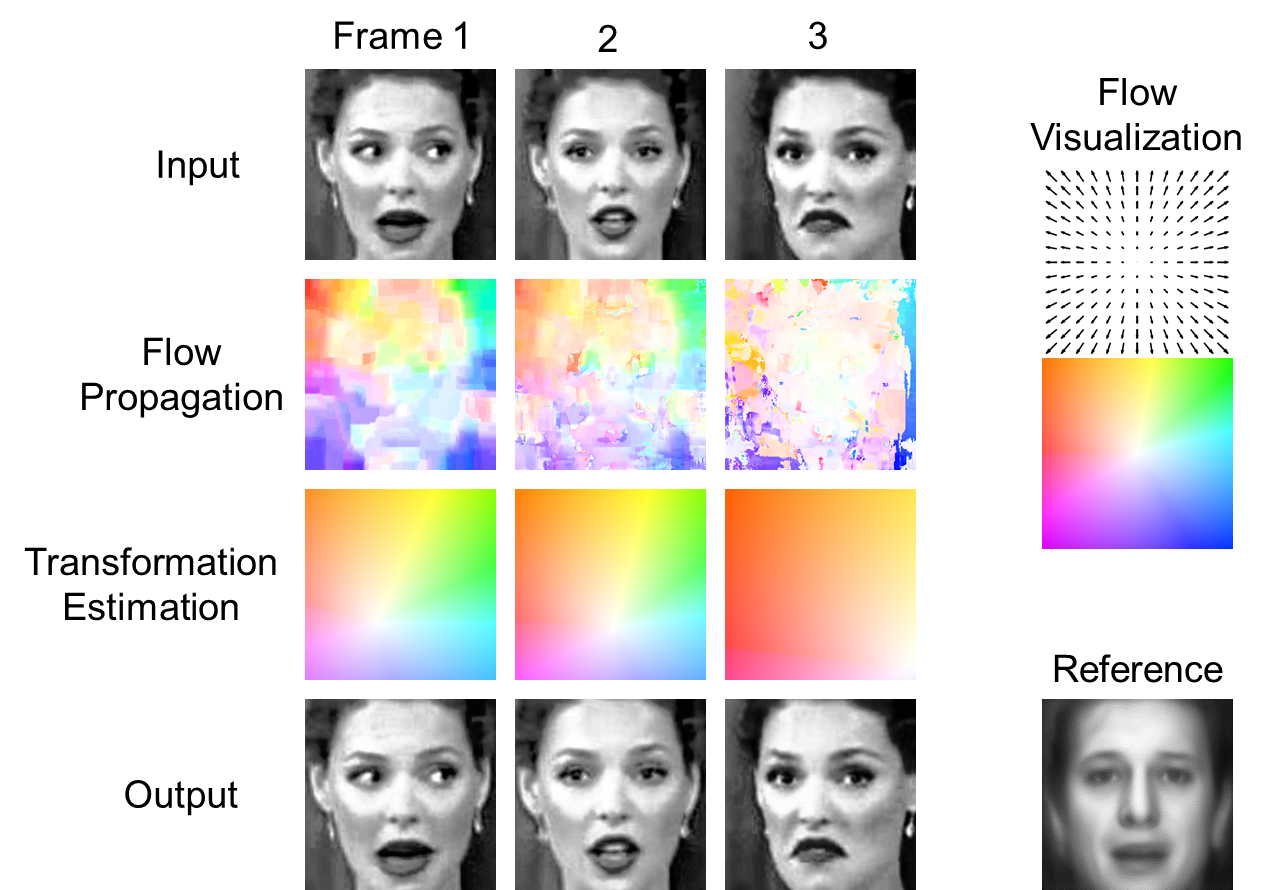
\includegraphics[width=\columnwidth]{fig/theory_example.png}
	\caption{Registration Example. The input sequence is registered with respect to the reference frame shown in bottom right. The flow visualization is coded as in \cite{Baker_ICCV07}. Better viewed in color.}
	\label{fig_theory_example}
\end{figure}

A registration example for face is visualized in Fig. \ref{fig_theory_example}. The flow propagation in Eq. \ref{eq:final}, i.e., $(1+\alpha+\beta)^{-1}(f_s^{i-1}+f_o^{i-1,i}+\frac{\alpha}{H}\sum_{j=1}^H(f_s^{i-j}+f_o^{i-j,i})+\beta{p})$, is visualized in the second row for consecutive frames. The affine transformation is then robustly estimated for each frame. The output sequence are registered with respect to the reference frame and exemplar frames comply with smoothness constraint. 


\subsection{\label{sec:details}Error Propagation and Closed-loop Rectification}

In our model, we sacrifice model optimality to efficient implementation. Therefore, the average registration error accumulates with time. The registration error is defined as the deviation from the canonical reference frame. Since we care about structural similarity, we compute the mean length of the SIFT flow from the current frame to the reference frame. For error analysis, we need videos with length of more than one minute ($1800$ frames in our case with $30$ fps) to observe the noticeable cumulative error. Therefore, we register a long sequence from Youtube and plot the error in Fig.\ref{fig_error_prop}. Although this error measurement consists of both global rigid head motion and local non-rigid muscle motion, we are still able to observe the error accumulation effect.

\begin{figure}[htbp]
	\centering
		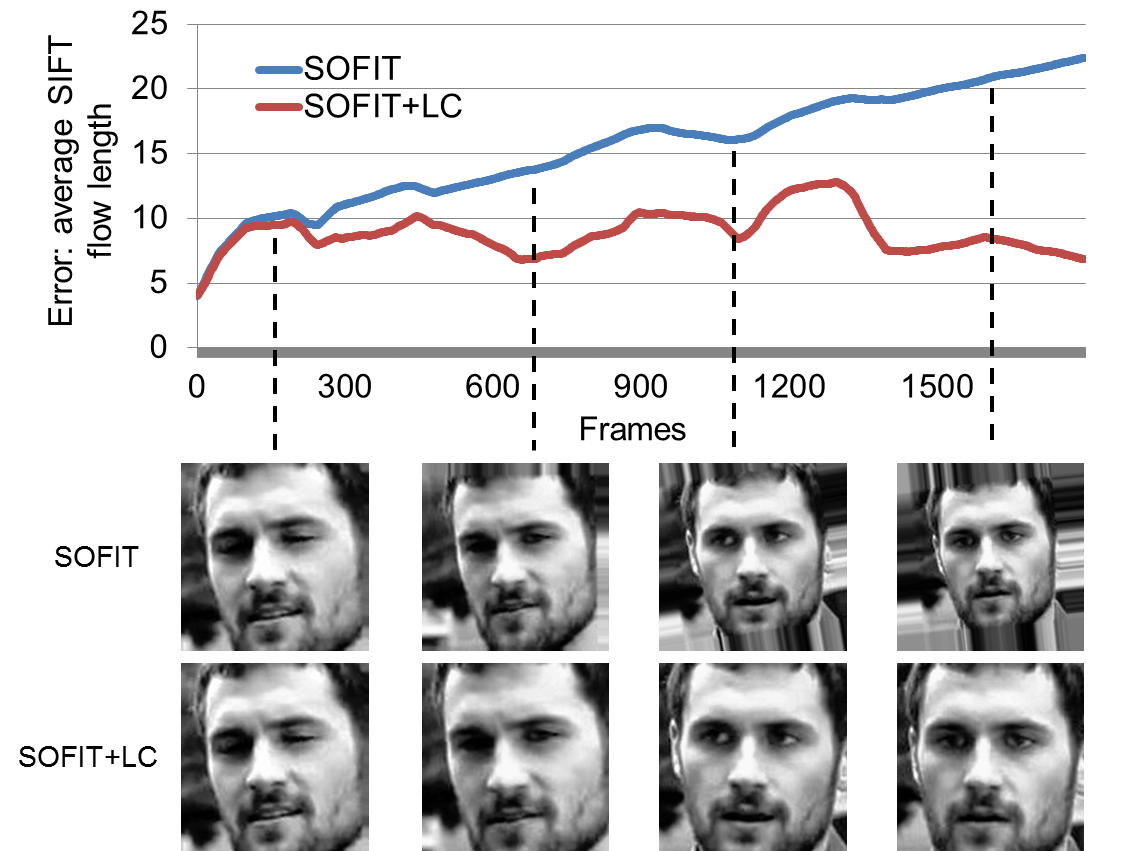
\includegraphics[width=\columnwidth]{fig/error_prop.png}
	\caption{The error accumulation with respect to time. The error is defined as the SIFT flow of the current frame to the canonical reference frame. We use loop-closure (LC) to update the global flow estimation and rectify the error. The LC is carried out every $300$ frames in this experiment.}
	\label{fig_error_prop}
\end{figure}

To solve this issue, we intend to update the global estimation at a certain rate without affecting the propagation computation. Inspired by the loop-closure strategy in robotics \cite{close_loop_icra_05}, we update $fs$ in Eq. \ref{eq:final} by recomputing the SIFT flow every $300$ frames. This update frequency is chosen because cumulative error is negligible in the $300$ frames, and this also provides enough time for $fs$ to be updated in parallel and will not affect the overall flow propagation. As seen in Fig. \ref{fig_error_prop}, the error is rectified due to this global flow estimation update. 


\subsection{\label{sec:time}Computational Cost Analysis}
We obtain considerable speedup from dynamic programming implementation for Eq. \ref{eq:final}. In essence, the SIFT flow only needs to be computed for the initialization. The steps to be carried out for every subsequent frame are the following:
\begin{enumerate}
\item Compute the dense optical flow with respect to the previous $H$ frame in parallel
\item Estimate affine transformation matrix using Eq. \ref{eq:final} based on the update coordinate value.
\end{enumerate}

We adopt the optical flow in OpenCV~\cite{opencv}. \Songfan{The aforementioned steps can be finished in approximately $47$ms on average for a $100\times100$ image on a quad-core Intel i7 4GHz machine with 32GB memory. In other words, the execution speed reaches 21 fps under this setting. }Since the bottleneck of our method is optical flow computation, one can further speedup the algorithm by GPU implementation. The initialization takes on the average \Songfan{$1.2$} second using the aforementioned settings. The computation is SIFT flow and optical flow are also in parallel. The loop-closure re-initialization is also in parallel with the the optical flow computation, and it will not affect the speed of the registration. 


%---------------------------------------------------------------
\section{\label{sec:experiment}Experimental Results}

\Songfan{In this section, we show results on facial action unit detection, vehicle recognition recognition, and image super-resolution. We have also included qualitative results on a range of classes of objects to demonstrate the generalizability of our approach.}

\subsection{Facial Action Unit Recognition}

We demonstrate SOFIT face registration technique by facial action unit (AU) recognition on FERA Challenge dataset~\cite{FERA11}. The goal of AU recognition is to detect $12$ frequently occurring AUs on a per-frame basis. We use the same protocol as the Facial Expression Recognition and Analysis Challenge (FERA2011)~\cite{Valstar_FERA11} AU sub-challenge. The data we use for training is the GEMEP-FERA training dataset, which includes 87 sequences and around 5400 frames. The pose and gesture of the subjects in this dataset are uncontrolled, and therefore, this dataset is more realistic and complex compared to MMI~\cite{Pantic_ICME05} and CK+~\cite{Kanade_FG00} datasets.

The main concerns here are two folds:
\begin{enumerate}
\item Is registration really an important issue in real-world AU recognition in uncontrolled environment?
\item If yes, can we improve the recognition performance just by adopting a better registration algorithm, i.e., SOFIT?
\end{enumerate}

To address these issues, we use the exact same feature as the baseline approach for better comparison. The only variable in our experiment design is using different registration methods. The baseline registration method detects both eye locations of the face, scale, and in-plane rotate the face. This registration belongs to in-plane image transformation category as summarized in \cite{Yang_SMCB12}. The state-of-the-art registration technique is called Emotion Avatar Image (EAI)~\cite{Yang_SMCB12}. It is another variation of SIFT flow method~\cite{Liu_PAMI11}. We have also included our earlier registration work \cite{Yang_FG13} for comparison.


\begin{table}[htbp]
\caption{Person-independent AUC-score result on FERA-GEMEP AU training set. Feature: Local Binary Pattern}
\begin{center}
\label{table:fera_lbp}
\begin{tabular}{|c|cccc|}
\hline
& \pbox{10cm}{Baseline \\\cite{Valstar_FERA11}}	&\pbox{10cm}{EAI \\\cite{Yang_SMCB12}}	&\pbox{10cm}{SOFAIT \\\cite{Yang_FG13}}	&\pbox{10cm}{SOFIT}	\\ \hline
AU1		&0.69	&0.68	&0.73	&\textbf{0.76}\cellcolor[gray]{0.9}	\\ 
AU2		&0.69	&0.68	&0.68	&\textbf{0.70}\cellcolor[gray]{0.9}	\\
AU4		&0.58	&\textbf{0.68}\cellcolor[gray]{0.9}	&0.66	&0.62 \\
AU6		&0.68	&0.69	&\textbf{0.79}\cellcolor[gray]{0.9}	&0.78	\\
AU7		&0.61	&0.62	&\textbf{0.75}\cellcolor[gray]{0.9}	&0.67 \\
AU10	&0.68	&0.61	&0.69	&\textbf{0.70}\cellcolor[gray]{0.9} \\
AU12	&0.68	&0.75	&\textbf{0.75}\cellcolor[gray]{0.9}	&0.74 \\
AU15	&0.52	&0.54	&0.65	&\textbf{0.69}\cellcolor[gray]{0.9} \\
AU17	&0.61	&0.66	&\textbf{0.71}\cellcolor[gray]{0.9}	&0.69 \\
AU18	&0.57	&0.72	&0.72	&\textbf{0.74}\cellcolor[gray]{0.9} \\
AU25	&0.53	&0.55	&\textbf{0.67}\cellcolor[gray]{0.9}	&0.57 \\
AU26	&0.52	&0.56	&\textbf{0.59}\cellcolor[gray]{0.9}	&0.58 \\ \hline
average	&0.61	&0.64	&\textbf{0.70}\cellcolor[gray]{0.9}	&0.69 \\ \hline

\end{tabular}
\end{center}
\end{table}


\begin{table}[htbp]
\caption{Person-independent AUC-score result on FERA-GEMEP AU training set. Feature: Local Phase Quantization}
\begin{center}
\label{table:fera_lpq}
\begin{tabular}{|c|cccc|}
\hline
& \pbox{10cm}{Baseline \\\cite{Valstar_FERA11}}	&\pbox{10cm}{EAI \\\cite{Yang_SMCB12}}	&\pbox{10cm}{SOFAIT \\\cite{Yang_FG13}}	&\pbox{10cm}{SOFIT}	\\ \hline
AU1		&0.67	&0.67	&0.72	&\textbf{0.77} \cellcolor[gray]{0.9}\cellcolor[gray]{0.9}	\\
AU2		&0.63	&0.69	&\textbf{0.70}\cellcolor[gray]{0.9}	&0.69	\\
AU4		&0.57	&0.55	&0.65	&\textbf{0.67}\cellcolor[gray]{0.9}	\\
AU6		&0.78	&0.74	&0.79	&\textbf{0.81}\cellcolor[gray]{0.9}	\\
AU7		&0.61	&0.58	&0.66	&\textbf{0.73}\cellcolor[gray]{0.9}	\\
AU10	&0.61	&0.65	&0.70	&\textbf{0.73}\cellcolor[gray]{0.9}	\\
AU12	&0.76	&0.78	&0.78	&\textbf{0.81}\cellcolor[gray]{0.9}	\\
AU15	&0.56	&0.65	&0.62	&\textbf{0.69}\cellcolor[gray]{0.9}	\\
AU17	&0.64	&0.63	&0.66	&\textbf{0.68}\cellcolor[gray]{0.9}	\\
AU18	&0.72	&0.74	&\textbf{0.76}\cellcolor[gray]{0.9}	&0.73	\\
AU25	&0.53	&0.54	&0.56	&\textbf{0.64}\cellcolor[gray]{0.9}	\\
AU26	&0.53	&0.54	&\textbf{0.63}\cellcolor[gray]{0.9}	&0.59	\\	\hline
average	&0.63	&0.65	&0.69	&\textbf{0.71}\cellcolor[gray]{0.9}	\\	\hline

\end{tabular}
\end{center}
\end{table}



The feature extraction and classification are conducted the same as the baseline approach. After we extracted the face from Viola-Jones face detector~\cite{Viola_IJCV04}, we resize them to $100\times100$ images and register them using the proposed method. Subsequently, we divide the image into $10\times10$ blocks, where the same type of Local Binary Pattern (LBP)~\cite{Ojala_PAMI02} texture feature for each block is computed and concatenated. We then train $12$ linear SVM binary classifiers based on the implementation of~\cite{SVMlib}, each of which is trained independently regardless of the co-occurrence of AUs.


For registration methods with reference frame, i.e., EAI \cite{Yang_SMCB12}, SOFAIT \cite{Yang_FG13}, and SOFIT, we use the level-1 Avatar Reference \cite{Yang_SMCB12} generated from FERA Challenge training data \cite{FERA11}. In generating a EAI representation, we need to select a temporal length parameter. The authors of the original EAI paper~\cite{Yang_SMCB12} choose the length of a single video (around $2$ seconds) for this parameter for facial expression recognition on a per-video basis. To generalize this registration technique in AU recognition on a per-frame basis, we heuristically determine the best value for the temporal length parameter. We carry out a leave-one-subject-out cross validation on the FERA-AU training data, and determine the parameter value to be $0.56$ second for the best F1 score over all AUs. This means for each frame in a video, approximately $14$ closest frames will be used to compute EAI representation. For the boundary frames, i.e. the starting and ending $7$ frames, we simply assign their values to be the $8$th frame from the beginning and the $8$th from the end, respectively. Thereafter, the aforementioned features are extracted from the EAI representations.

\begin{figure*}[t]
	\centering
		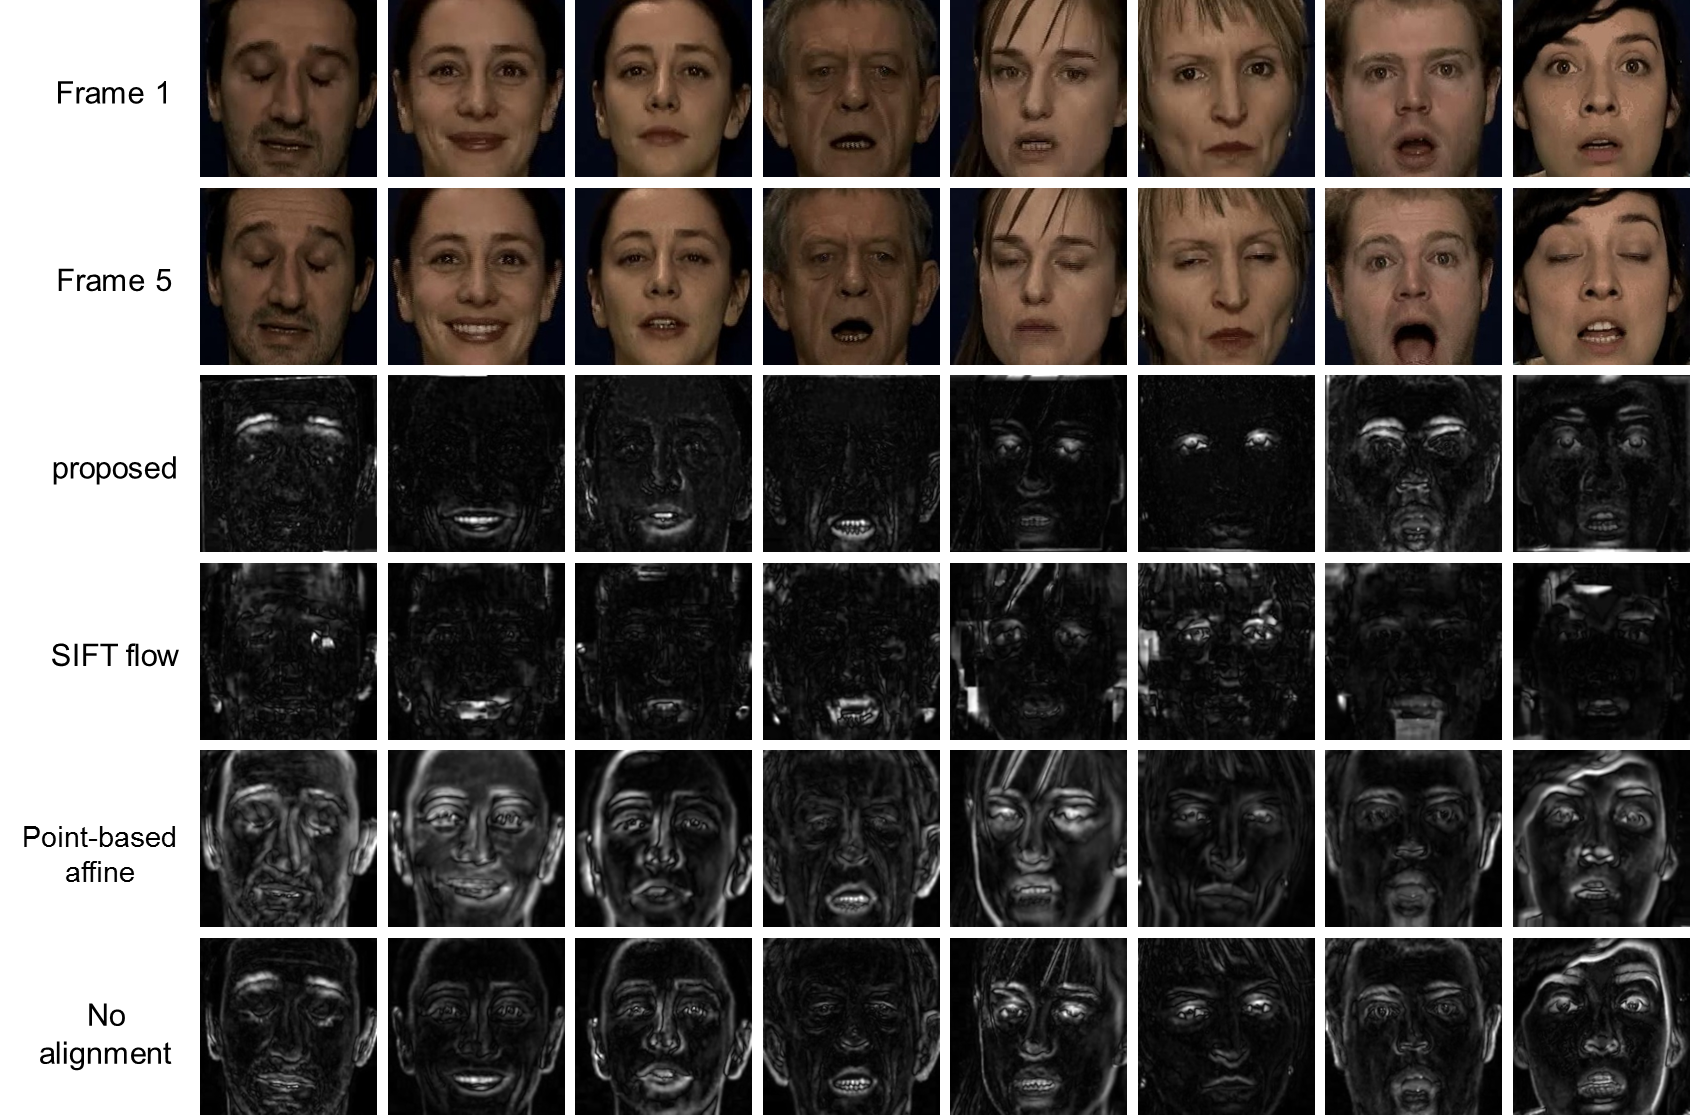
\includegraphics[width=0.8\textwidth]{fig/fera_diff.png}
	\caption{Qualitative result comparison. Row 1 and 2 are the first and fifth frame of a sequence. Row 3 to 5 are the cumulative absolute frame difference of 5 unaligned frames using method SOFIT, SIFT flow~\cite{Liu_PAMI11}, point-based affine where points are detected using deformable part-based model (DPM)~\cite{Zhu_CVPR12}, respectively. Row 6 are without alignment. The proposed alignment technique captures the correct non-rigid motion of face, for example, eyebrows raise for first column and mouth open for second column.}
	\label{fig:fera_diff}
\end{figure*}


\begin{figure}[htbp]
	\centering
		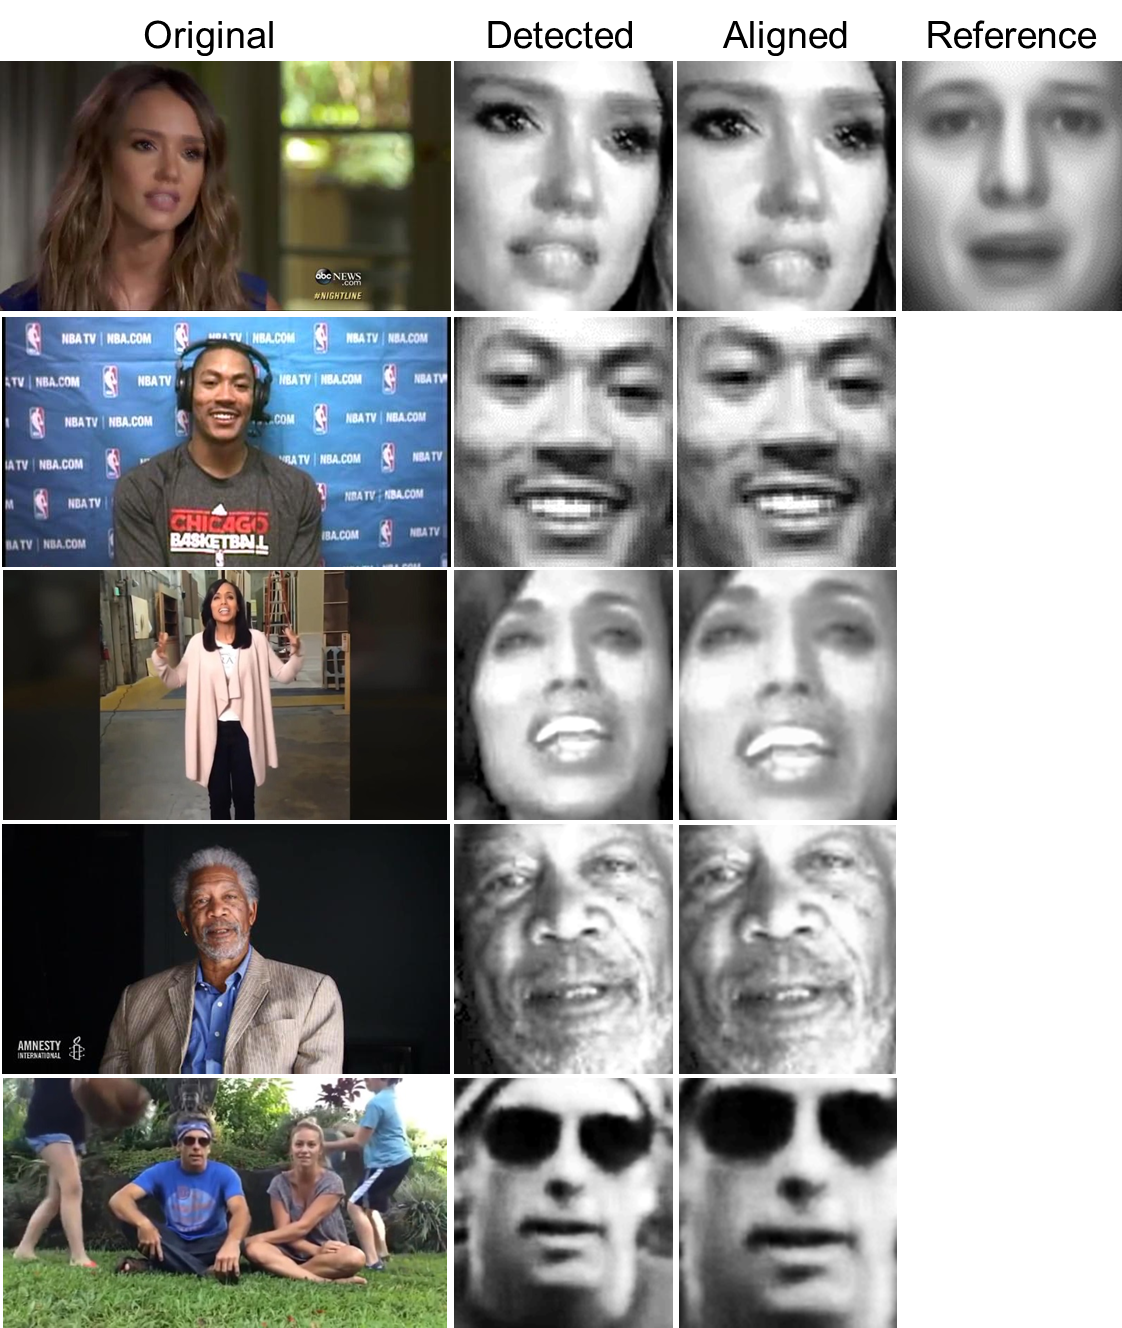
\includegraphics[width=.8\columnwidth]{fig/suppliment.png}
	\caption{More face alignment results using SOFIT. Due to aligning with canonical reference face, all pose rotations, translations, and scales are rectified. }
	\label{fig:suppliment}
\end{figure}


\begin{figure*}[htbp]
	\centering
 \subfigure[First row: first frame without alignment; second row: the average of individual frames aligned by SOFIT]{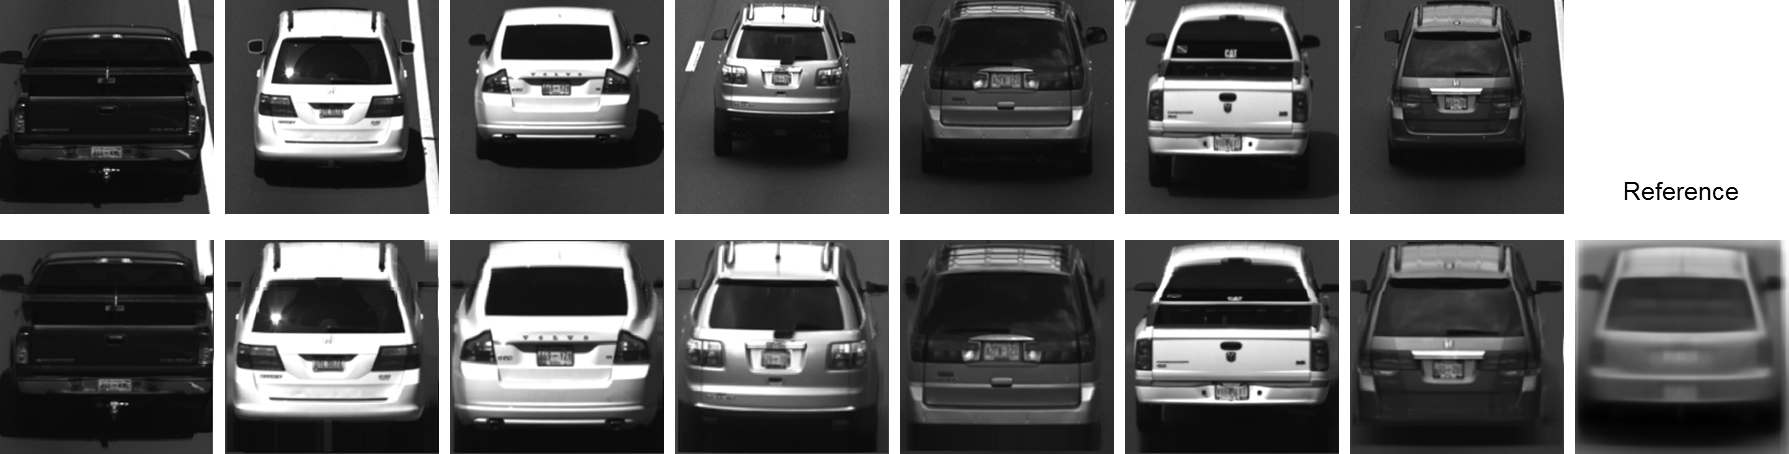
\includegraphics[width=.8\textwidth ]{fig/m3_over_m1.png}}

 \subfigure[First row: first frame aligned by SIFT-flow affine; second row: the average of individual frames aligned by SOFIT]{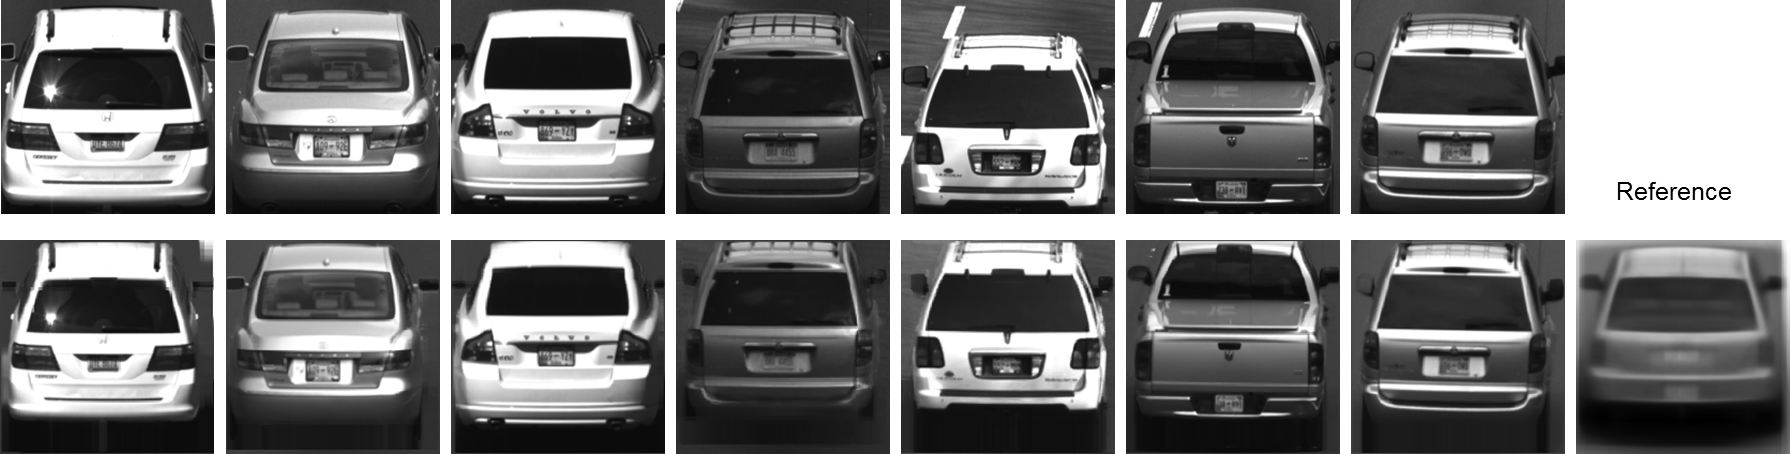
\includegraphics[width=.8\textwidth ]{fig/m3_over_m2.png}}

	\caption{Sample registration results. The first row of both (a) and (b) are misclassified examples by SVM while the second row are correctly classified. In (a), SOFIT is able to align detected vehicles to a similar scale. In (b), SOFIT mainly corrects the missing bottom and align similar parts of the vehicle according to their structure. The bottom right shows the avatar reference frame generated by~\cite{Yang_SMCB12} used in the initialization step.}
	\label{fig:vehicle_reg_sample}
\end{figure*}


\begin{figure*}[htbp]
	\centering
		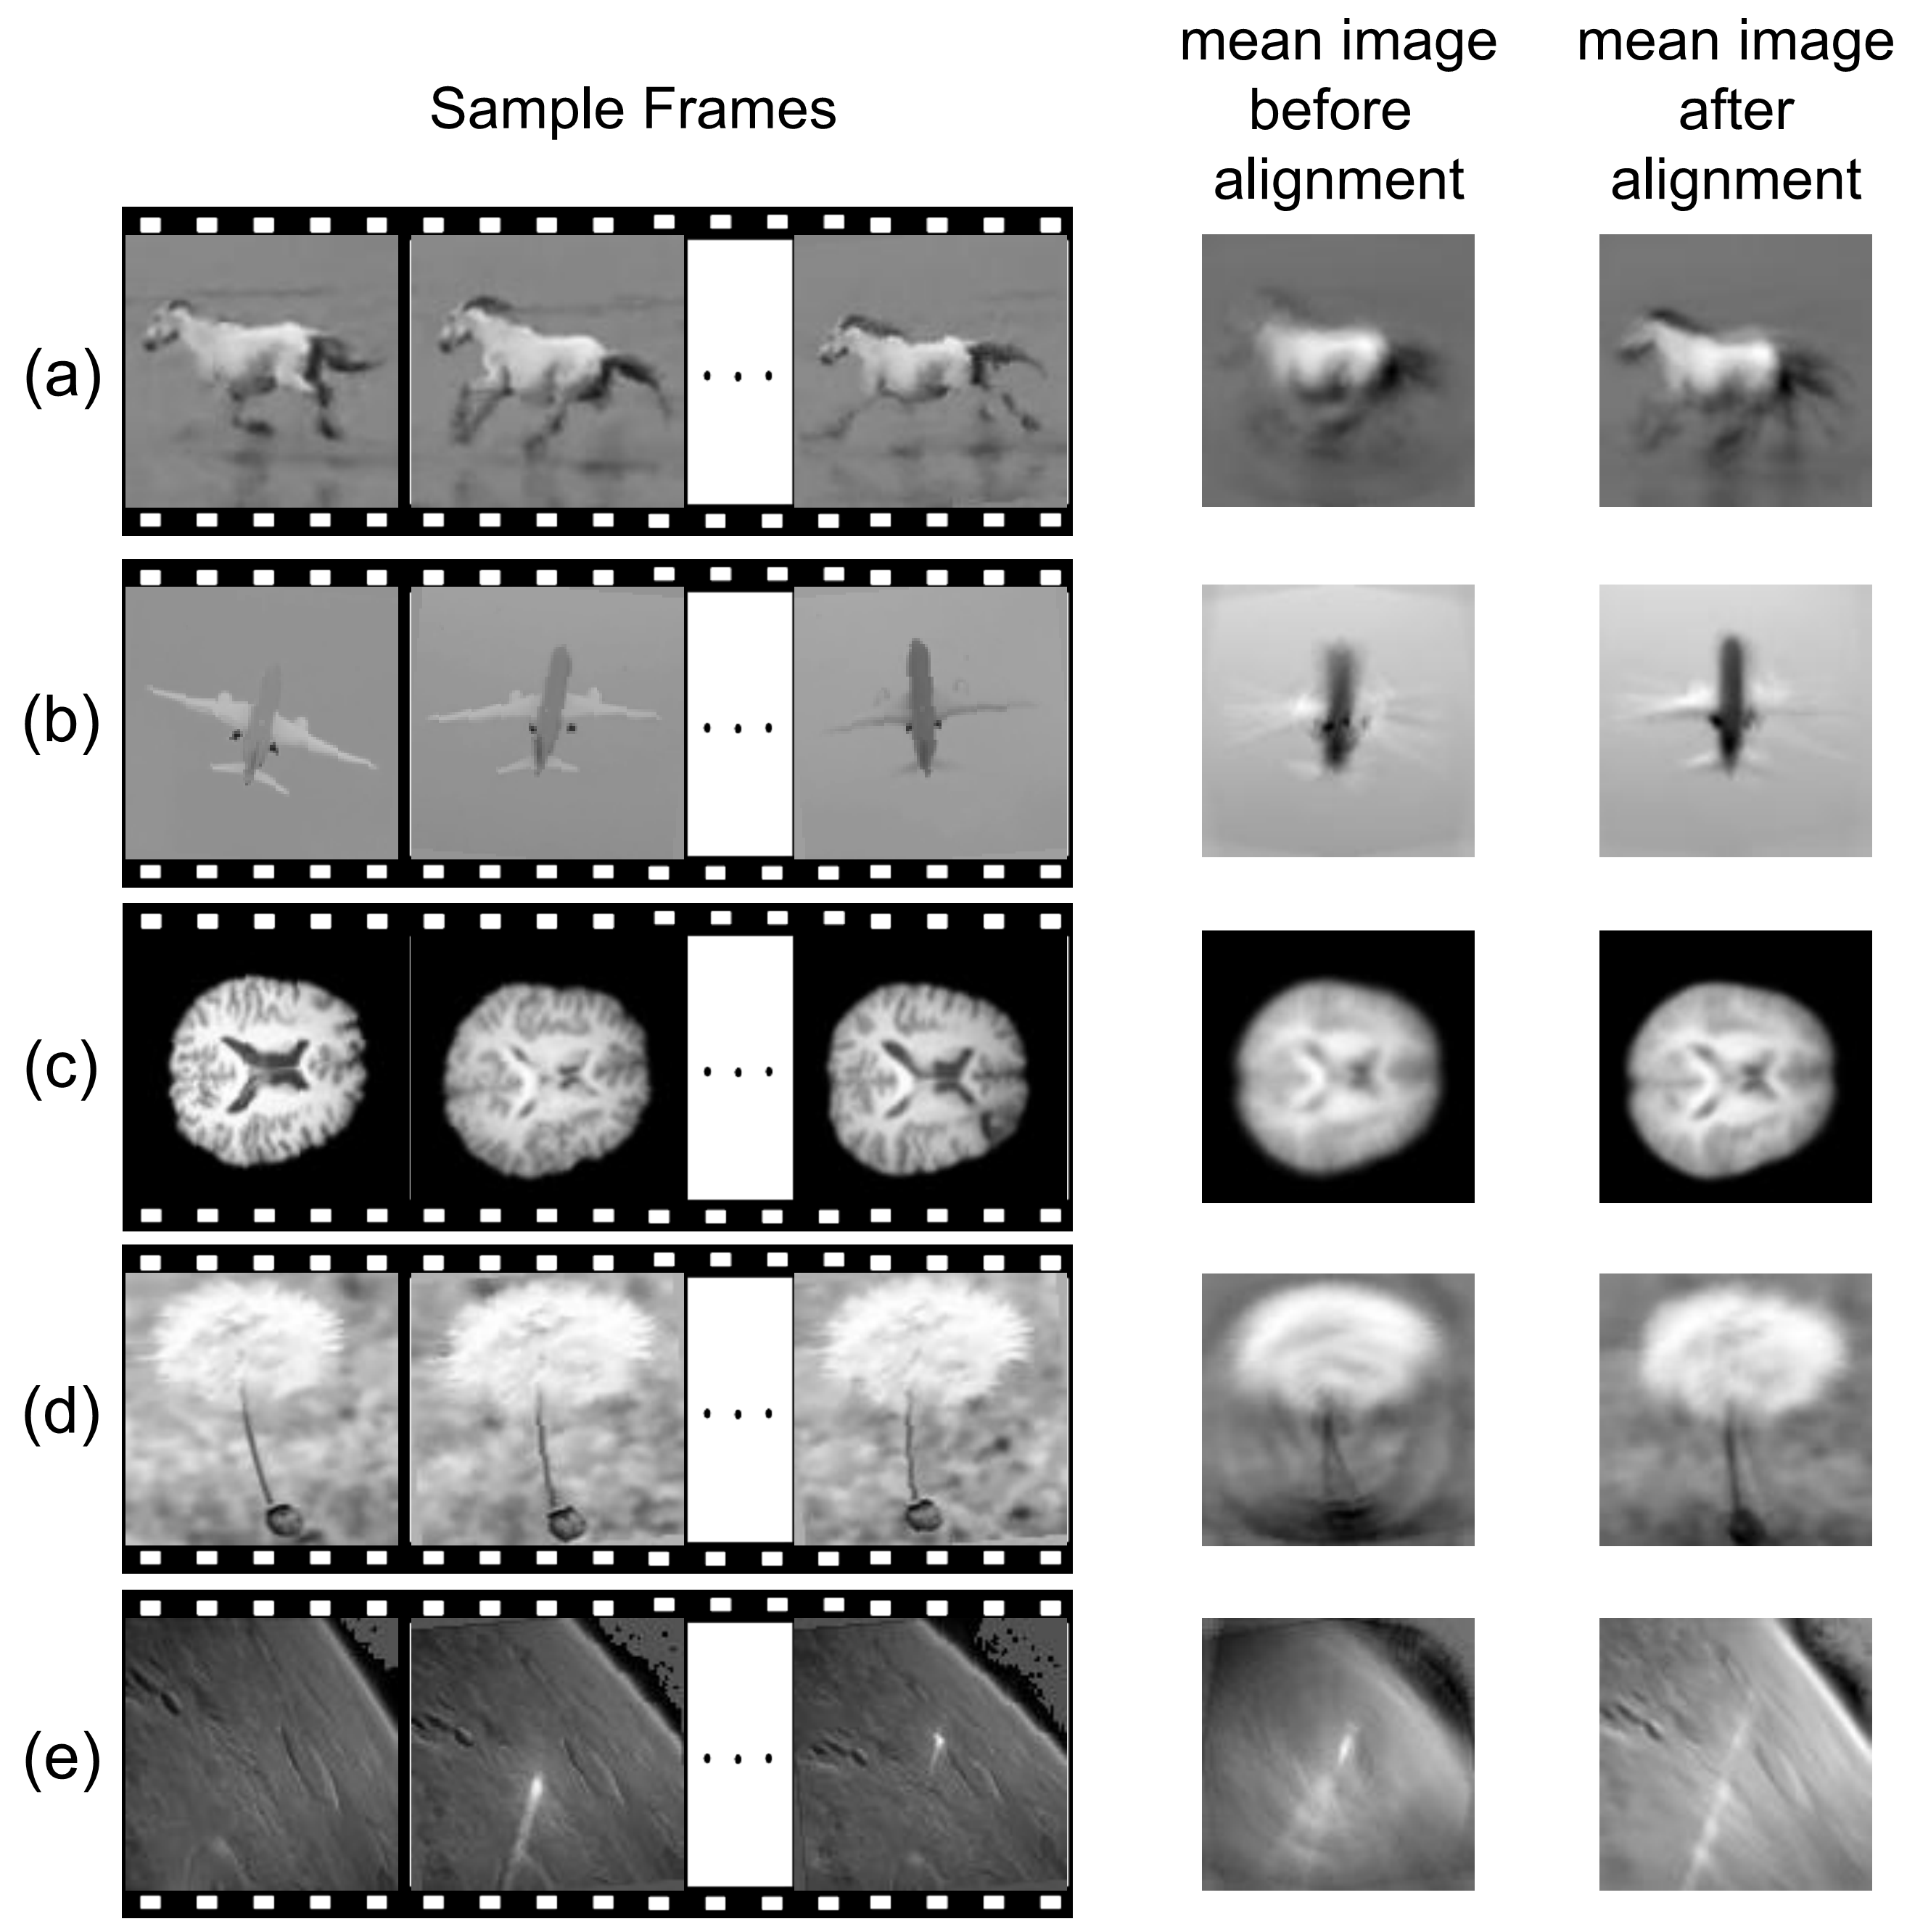
\includegraphics[width=.65\textwidth]{fig/object_ex.png}
	\caption{\Songfan{More registration results using SOFIT for generic objects in video, each row of which represents challenges in different aspects. There are approximately 50 images per sequence and the reference frame is randomly selected from the sequence. The averages of each sequence before/after SOFIT alignment are shown in the last two columns. (a) Non-rigid motion, mainly found by the poses of horse. (b) In-plane and out-of-plane rotation. (c) Appearance variation. This row contains Magnetic Resonance Imaging (MRI) samples from different individuals. Though it is not strictly video per se, the results show that our method is robust against intensity variations. (d) Cluttered background. (e) Outliers. While the camera is non-stationary, there is a rocket moving against the Mars. Since we explicitly model the dominant motion of the scene, outliers (such as the rocket) have little impact on the alignment results.}}
	\label{fig:object_ex}
\end{figure*}

Since the ground-truth label is only available for the FERA-AU training set, we carried out a person-independent cross validation experiment, where no test subject is used for training, and the average performance is reported. Due to the finite scale of the training exemplars, person-independent test is essential to demonstrate the generalization ability of an approach to unseen subjects. Table \ref{table:fera_lbp} and \ref{table:fera_lpq} shows the performance measured by local binary pattern (LBP) and local phase quantization (LPQ). The score is area under curve (AUC) of the receiver operating characteristic (ROC) curve. As seen from Table \ref{table:fera_lbp} and \ref{table:fera_lpq}, SOFIT and SOFAIT outperform the baseline and EAI registration method. Although EAI performs well in discrete emotion recognition \cite{Yang_SMCB12}, in a per-frame based setting, however, EAI lacks ability to reveal the subtle motion. When using LBP feature (Table \ref{table:fera_lbp}), SOFIT and SOFAIT are comparable and SOFIT performs better in the case of using LPQ (Table \ref{table:fera_lpq}). SOFIT with LPQ feature obtains the highest score in 9 out of 12 categories. 

We should point out that the video sequences in FERA-GEMEP is relatively short, i.e. around 2 seconds. Thus, the propagation error is not high and the appearance of registration results are similar using SOFIT and SOFAIT in most of the cases. In a longer video however, e.g., Fig. \ref{fig_error_prop}, the error of SOFAIT rises faster than SOFIT. Moreover, we also observe similar reference-independent effect as shown in \cite{Yang_FG13}, where is performance will not degenerate as the reference frame changes. 

Fig.~\ref{fig:fera_diff} shows the qualitative evaluation why our registration improves the baseline and EAI approaches. We compute the absolute frame difference of the first 5 frames for both unaligned and aligned faces. As shown in the third and fourth column of Fig.~\ref{fig:fera_diff}, the unaligned frame difference reveals motion mainly caused by the edge feature of a face, while after alignment, the non-rigid muscle motion is retained. We provide more visual alignment results on face in Fig.~\ref{fig:suppliment} and on general objects in Fig.~\ref{fig:object_ex}.



\subsection{Rear-view Vehicle Recognition}


In the application of surveillance and traffic monitoring, the ability to classify the type of a vehicle is essential for vehicle identification, circumventing problems such as license spoofing. Current work on vehicle recognition~\cite{Petrovic04}~\cite{Negri06}~\cite{Zafar09}~\cite{Pearce11} rely on license plate for alignment. Matching a video of an unknown vehicle with database faces various challenges such as view variation, illumination change, etc. Video data were collected from a camera mounted on top of a freeway lane over several days, during which 1664 vehicles were collected. The collected rear-view vehicle data fit in the context of our dense-flow based registration method, i.e., object shapes are similar and the structure/texture variation is key for recognition. 

Three individuals manually labeled four vehicle type, namely sedan, minivan, pickup, and SUV. The ground-truth is set to be the majority label by all three individuals. As some of the vehicles are hard to be identified, and there is a tie between different individuals (three different classes are picked by the three individuals), the data is not included. Finally 1505 vehicle with ground-truth label are used as our data for evaluation. Vehicle ROI were detected by the moving object detection method from~\cite{Thakoor05}. ROIs are then refined by removing shadows and enforcing bilateral symmetry~\cite{Thakoor13}. For each vehicle sequence, there are approximately 10 frames. Fig.~\ref{fig:vehicle_raw_data} shows a sample frame illustrating a detection result.  

\begin{figure}[htbp]
	\centering
		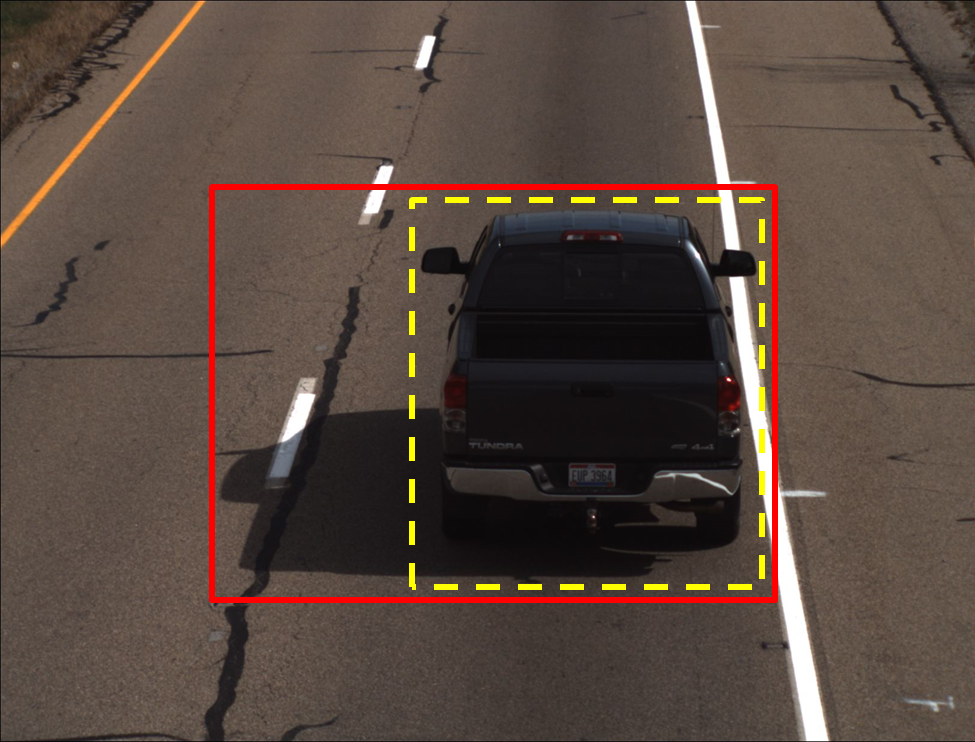
\includegraphics[width=.9\columnwidth]{fig/vehicle_raw_data.png}
	\caption{Sample vehicle detection result. Red rectangle is the result of vehicle ROI detection and yellow dash rectangle is the result after enforcing bilateral symmetry.}
	\label{fig:vehicle_raw_data}
\end{figure}

Due to our camera setup, the recorded vehicle is moving away from the scene. Therefore, we consider the first frame of the video as the frame where the vehicle is fully observed. As we can imagine, the first frame is the one with the best quality of the entire sequence. Three methods in comparison are used to generate image representation of ROIs from each video. (a) First frame without alignment, (b) First frame with SIFT-flow affine alignment (namely the initialization step of our approach), (c) The median representation of the entire sequence aligned using SOFIT. We demonstrate that by simply taking the mean of the entire aligned sequence, the representation is superior to just using a single frame. The reference frame in use is also the level-1 Avatar Reference generated by following \cite{Yang_SMCB12}. Again, it is essentially an image based summary of the entire vehicle in canonical appearance. Sample alignment results are shown in Fig. \ref{fig:vehicle_reg_sample}.

The ROIs are all resized to $200\times200$ for all three methods. The locally normalized Harris strength (LNHS) features~\cite{Pearce11} is used as the texture descriptor. We adopt the VLFeat~\cite{vlfeat} implementation for $\sigma=2.0$. The Harris strengths are split into $32\times32$ cells and normalized in $3\times3$ blocks. Descriptions are generated by shifting block by 1 pixel. We then use linear Support Vector Machine~\cite{sklearn} as the classifier without parameter tuning (i.e., $C=1.0$). A 10-fold cross validation is carried out and the result is reported in Fig~.\ref{fig:fig_vehicle_cls_f1}. The F1 score shows that SOFIT alignment is able to leverage image sequences and generate a robust representation for superior classification accuracy. 

\begin{figure}[htbp]
	\centering
		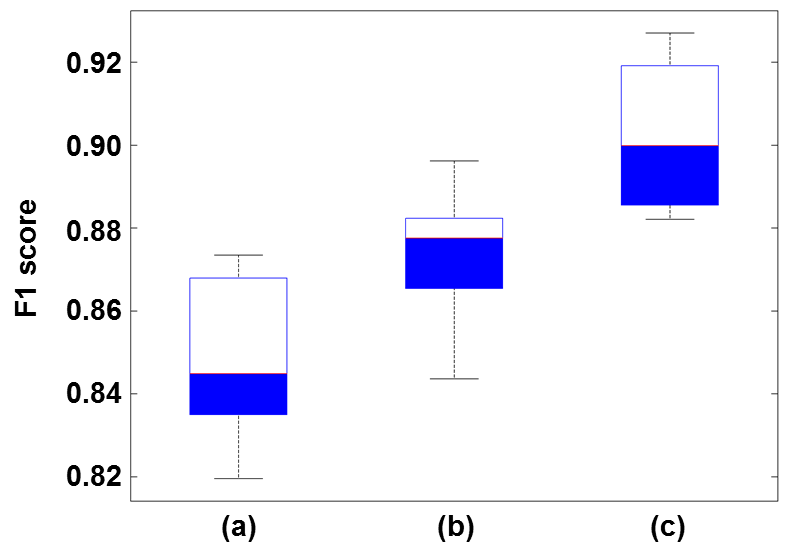
\includegraphics[width=.6\columnwidth]{fig/vehicle_cls_f1.png}
	\caption{The 10-fold cross validation results comparison for vehicle recognition shown by the boxplot. (a) unaligned, (b) aligned with initialization, (c) SOFIT.}
	\label{fig:fig_vehicle_cls_f1}
\end{figure}

\subsection{Multi-frame Image Super-resolution}

\begin{figure}[t]
	\centering
		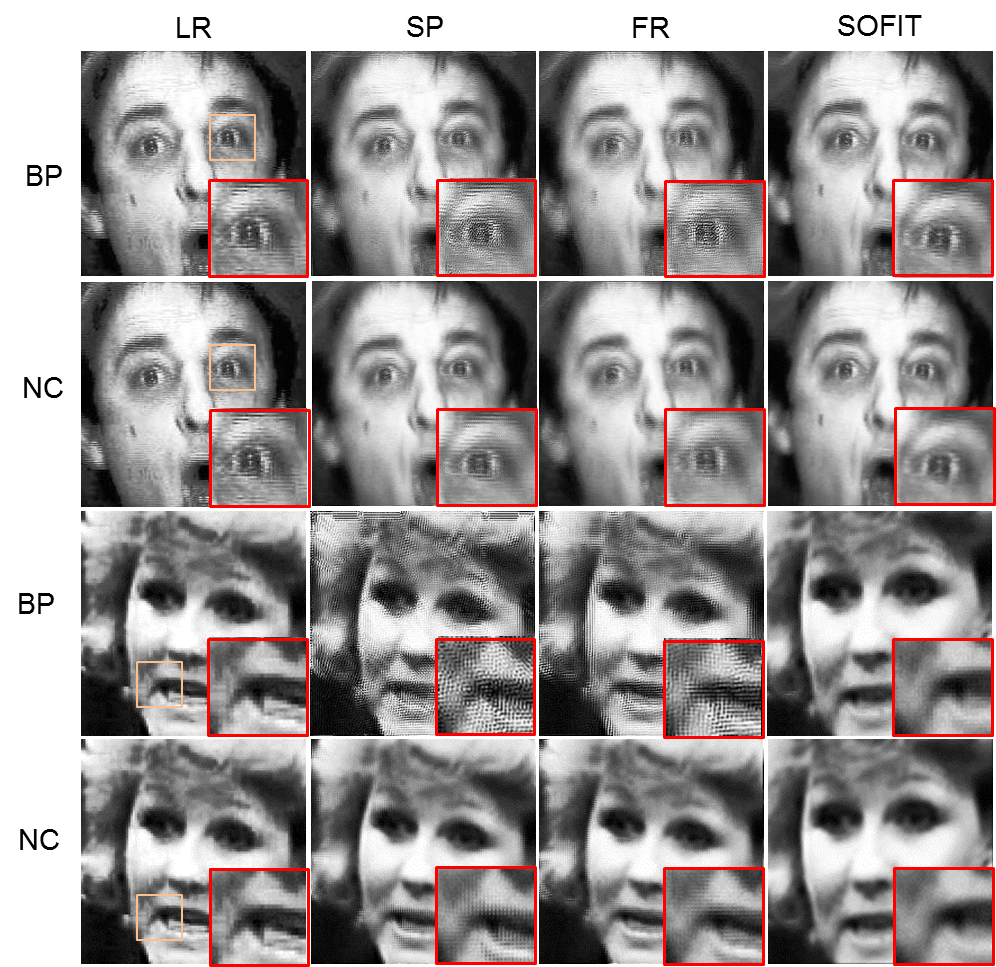
\includegraphics[width=\columnwidth]{fig/superResolution.png}
	\caption{Comparison of super-resolution results using different registration methods for 2 subjects. For each row from left to right: one of the LR inputs (enlarged by pixel replication), sub-pixel registration (SP)~\cite{Keren_CVPR88}, frequency domain based registration (FR)~\cite{Vandewalle06}, and the proposed registration method. We use two SR methods to reconstruct the high-resolution outputs: iterated back-projection (BP)~\cite{Irani91} and normalized convolution (NC)~\cite{Pham_06}. The red blocks show the magnified parts from the pink blocks.}
	\label{fig:superResolution}
\end{figure}

In the imaging process, it is common to acquire images with low-resolution (LR) and/or certain artifacts such as blurriness, noise, etc. Image super-resolution (SR) is the process of generating a high-resolution (HR) image from one or more low-resolution inputs. In the past few decades, there has been extensive work on super-resolution methods. Based on the inputs, the SR algorithms can be classified in two categories: single-image based~\cite{Sun_CVPR08} and multi-image based methods~\cite{Irani91}. We apply SOFIT registration algorithm proposed in this paper to generate aligned images as inputs to different multi-image based SR methods. Here we compare our registration method with two registration methods: frequency domain based method (FR)~\cite{Vandewalle06}, and registration using sub-pixel displacement (SP)~\cite{Keren_CVPR88}. These registration methods are then used in two SR methods: iterated back-projection (BP)~\cite{Irani91}, and normalized convolution based method (NC)~\cite{Pham_06}. Figure~\ref{fig:superResolution} shows the comparison of some sample results using different registration methods in different SR algorithms.

\begin{figure}[htbp]
	\centering
		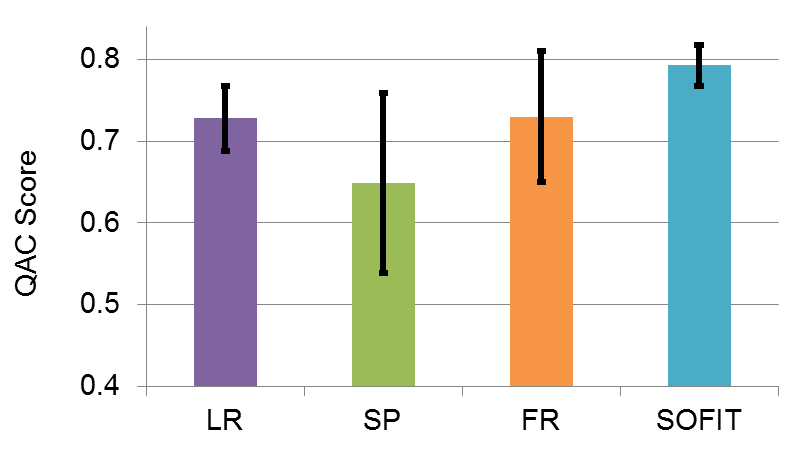
\includegraphics[width=.8\columnwidth]{fig/SR_quant.png}
	\caption{Image quality comparison between video-based super-resolution results and the proposed method. A recent non-reference image quality assessment method~\cite{Xue_CVPR13} is used. The higher the score, the better the estimated visual quality is. LR is low-resolution input images. SP denotes the super-resolved results using~\cite{Keren_CVPR88}. FR is the super-resolved results using~\cite{Vandewalle06}. These benchmark methods are compared with the proposed SOFIT method.}
	\label{fig:SR_quant}
\end{figure}

From Fig.~\ref{fig:superResolution} we see that with our registration method, the SR results are significantly improved over other SR methods in terms of visual quality. Despite the poor quality of the input frames, the results by our method are smooth with much fewer artifacts (e.g., noise, blockiness). The gain on the performance of SR directly comes from the accuracy of the proposed registration method. The output images by our methods are also well rectified which would be desirable for future processing purposes, such as AU and expression recognition. 

To quantitatively evaluate the image quality using our registration method, we compute a recent proposed non-reference image quality index, Quality-aware clustering (QAC)~\cite{Xue_CVPR13}, for output images using our method and competing super-resolution methods. QAC is a general purpose blind image quality assessment method that has high linearity to human perception of image quality. Fig.~\ref{fig:SR_quant} lists the average image quality scores on 87 sequences from GEMEP-FERA database~\cite{FERA11}. Compared to the LR input and output using different super-resolution methods, the output of SOFIT achieves the highest scores with lowest standard deviation, which indicates better visual quality through this general quantitative measure.

%
%comment: the qualitative result for face recognition is inferior than even with this registration. The reason is that this algorithm is designed for aligning local feature and non-rigid motion, as well as attenuate person-independent information. In the context of face recognition, the purpose is the opposite where person-independent information should be retained if not amplified.


\section{Conclusions\label{sec:conclusion}}

We developed a video-based real-time face registration technique, SOFIT, and demonstrate its applications in AU recognition, vehicle recognition, and image super-resolution. This approach utilizes holistic dense flow-based information, and therefore, it is robust to detection error and noise. Minor out-of-plane head rotation can also be corrected by employing structural information from SIFT flow. Besides, this method is able to generate temporally smooth registration results which are essential for spontaneous facial expression analysis and super-resolution. Last but not least, with the dynamic programming implementation, this method is suitable for real-time processing.


%\section{Acknowledgements}
%
%This material is based upon work supported by the National Science Foundation under Grant No.
%0727129 and 0915270.
%The authors would like to thank Dr. Michel Valstar from the University of Nottingham, the organizer of FERA 2011 Challenge, for evaluating the AU testing results.

% Can use something like this to put references on a page
% by themselves when using endfloat and the captionsoff option.
\ifCLASSOPTIONcaptionsoff
  \newpage
\fi



% trigger a \newpage just before the given reference
% number - used to balance the columns on the last page
% adjust value as needed - may need to be readjusted if
% the document is modified later
%\IEEEtriggeratref{8}
% The "triggered" command can be changed if desired:
%\IEEEtriggercmd{\enlargethispage{-5in}}

% references section

% can use a bibliography generated by BibTeX as a .bbl file
% BibTeX documentation can be easily obtained at:
% http://www.ctan.org/tex-archive/biblio/bibtex/contrib/doc/
% The IEEEtran BibTeX style support page is at:
% http://www.michaelshell.org/tex/ieeetran/bibtex/
%\bibliographystyle{IEEEtran}
% argument is your BibTeX string definitions and bibliography database(s)
%\bibliography{IEEEabrv,../bib/paper}
%
% <OR> manually copy in the resultant .bbl file
% set second argument of \begin to the number of references
% (used to reserve space for the reference number labels box)
\bibliographystyle{IEEEtran}
\bibliography{SOFA}


\begin{IEEEbiography}[{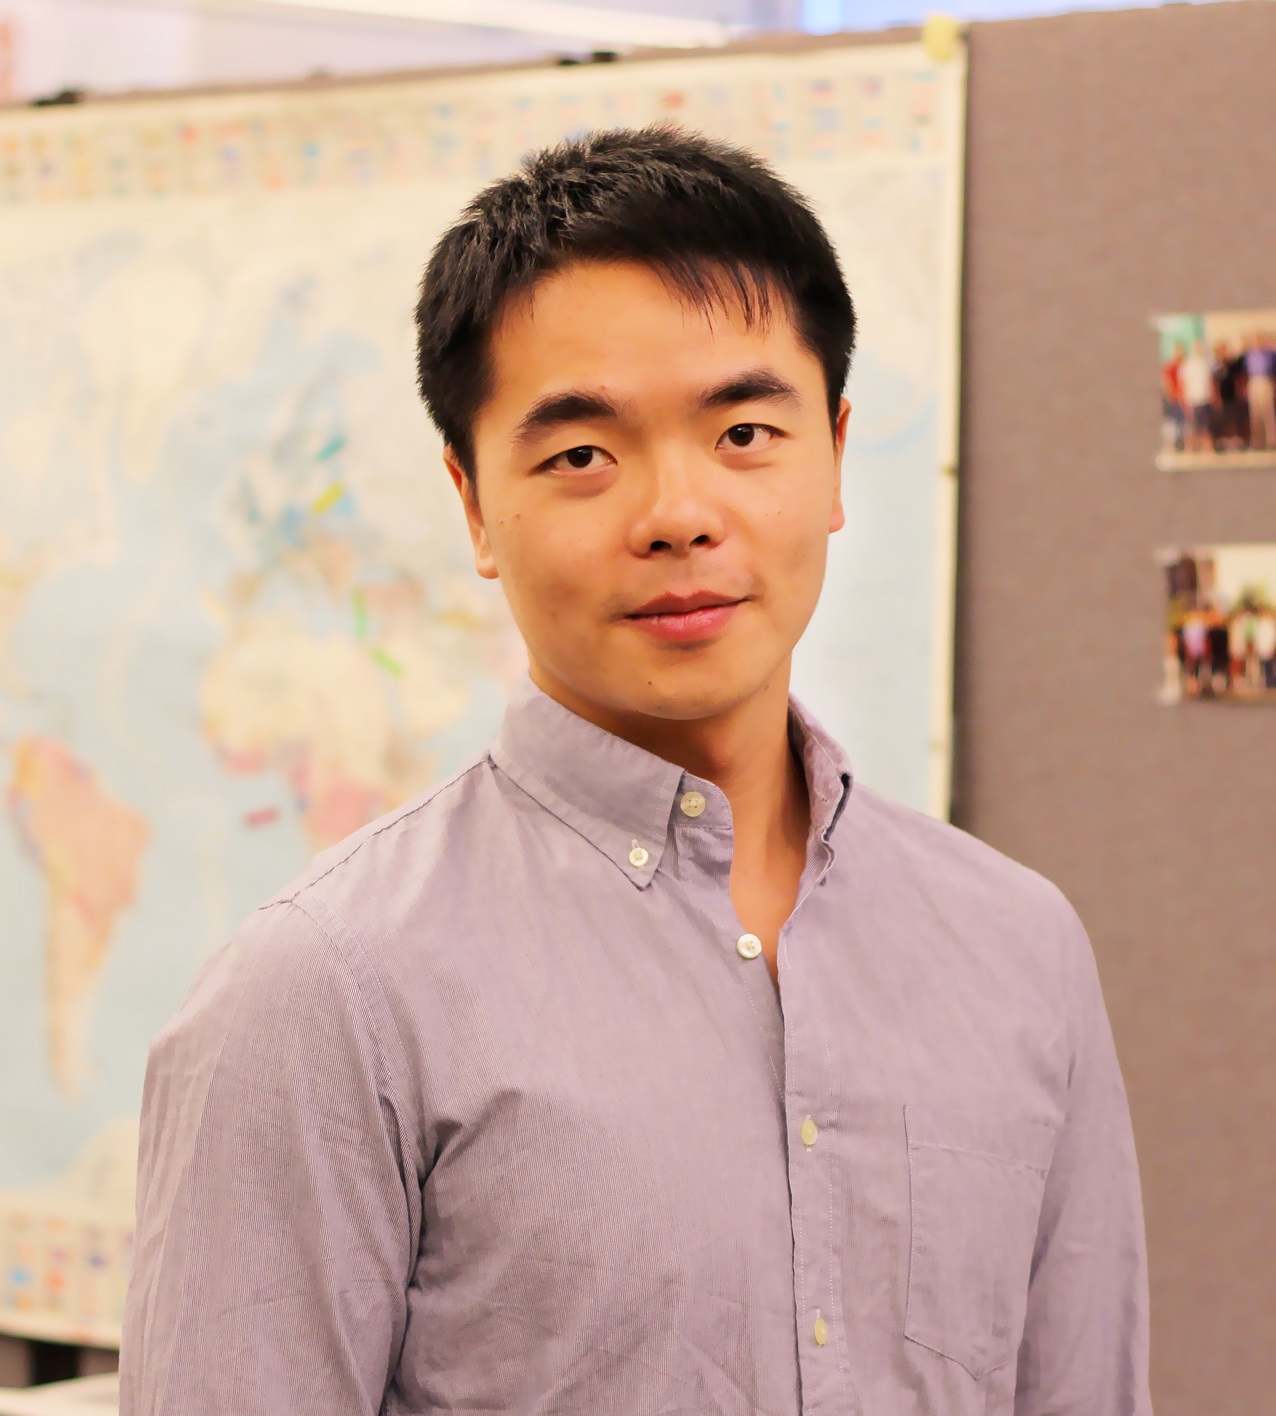
\includegraphics[width=1in,height=1.25in,clip,keepaspectratio]{pic/songfan.jpg}}]{Songfan Yang}
(S'10-M'14) received the B.S. degree in Electrical Engineering from Sichuan University, Chengdu, China, in 2009 and the M.S. and Ph.D. degree in Electrical Engineering from University of California, Riverside. He is currently an Associate Professor of College of Electronics and Information Engineering at Sichuan University. His research interests include computer vision, pattern recognition, and affective computing. He holds the Best Entry Award of the FG 2011 Facial Expression Recognition and Analysis emotion challenge (FERA) competition.
\end{IEEEbiography}

\begin{IEEEbiography}[{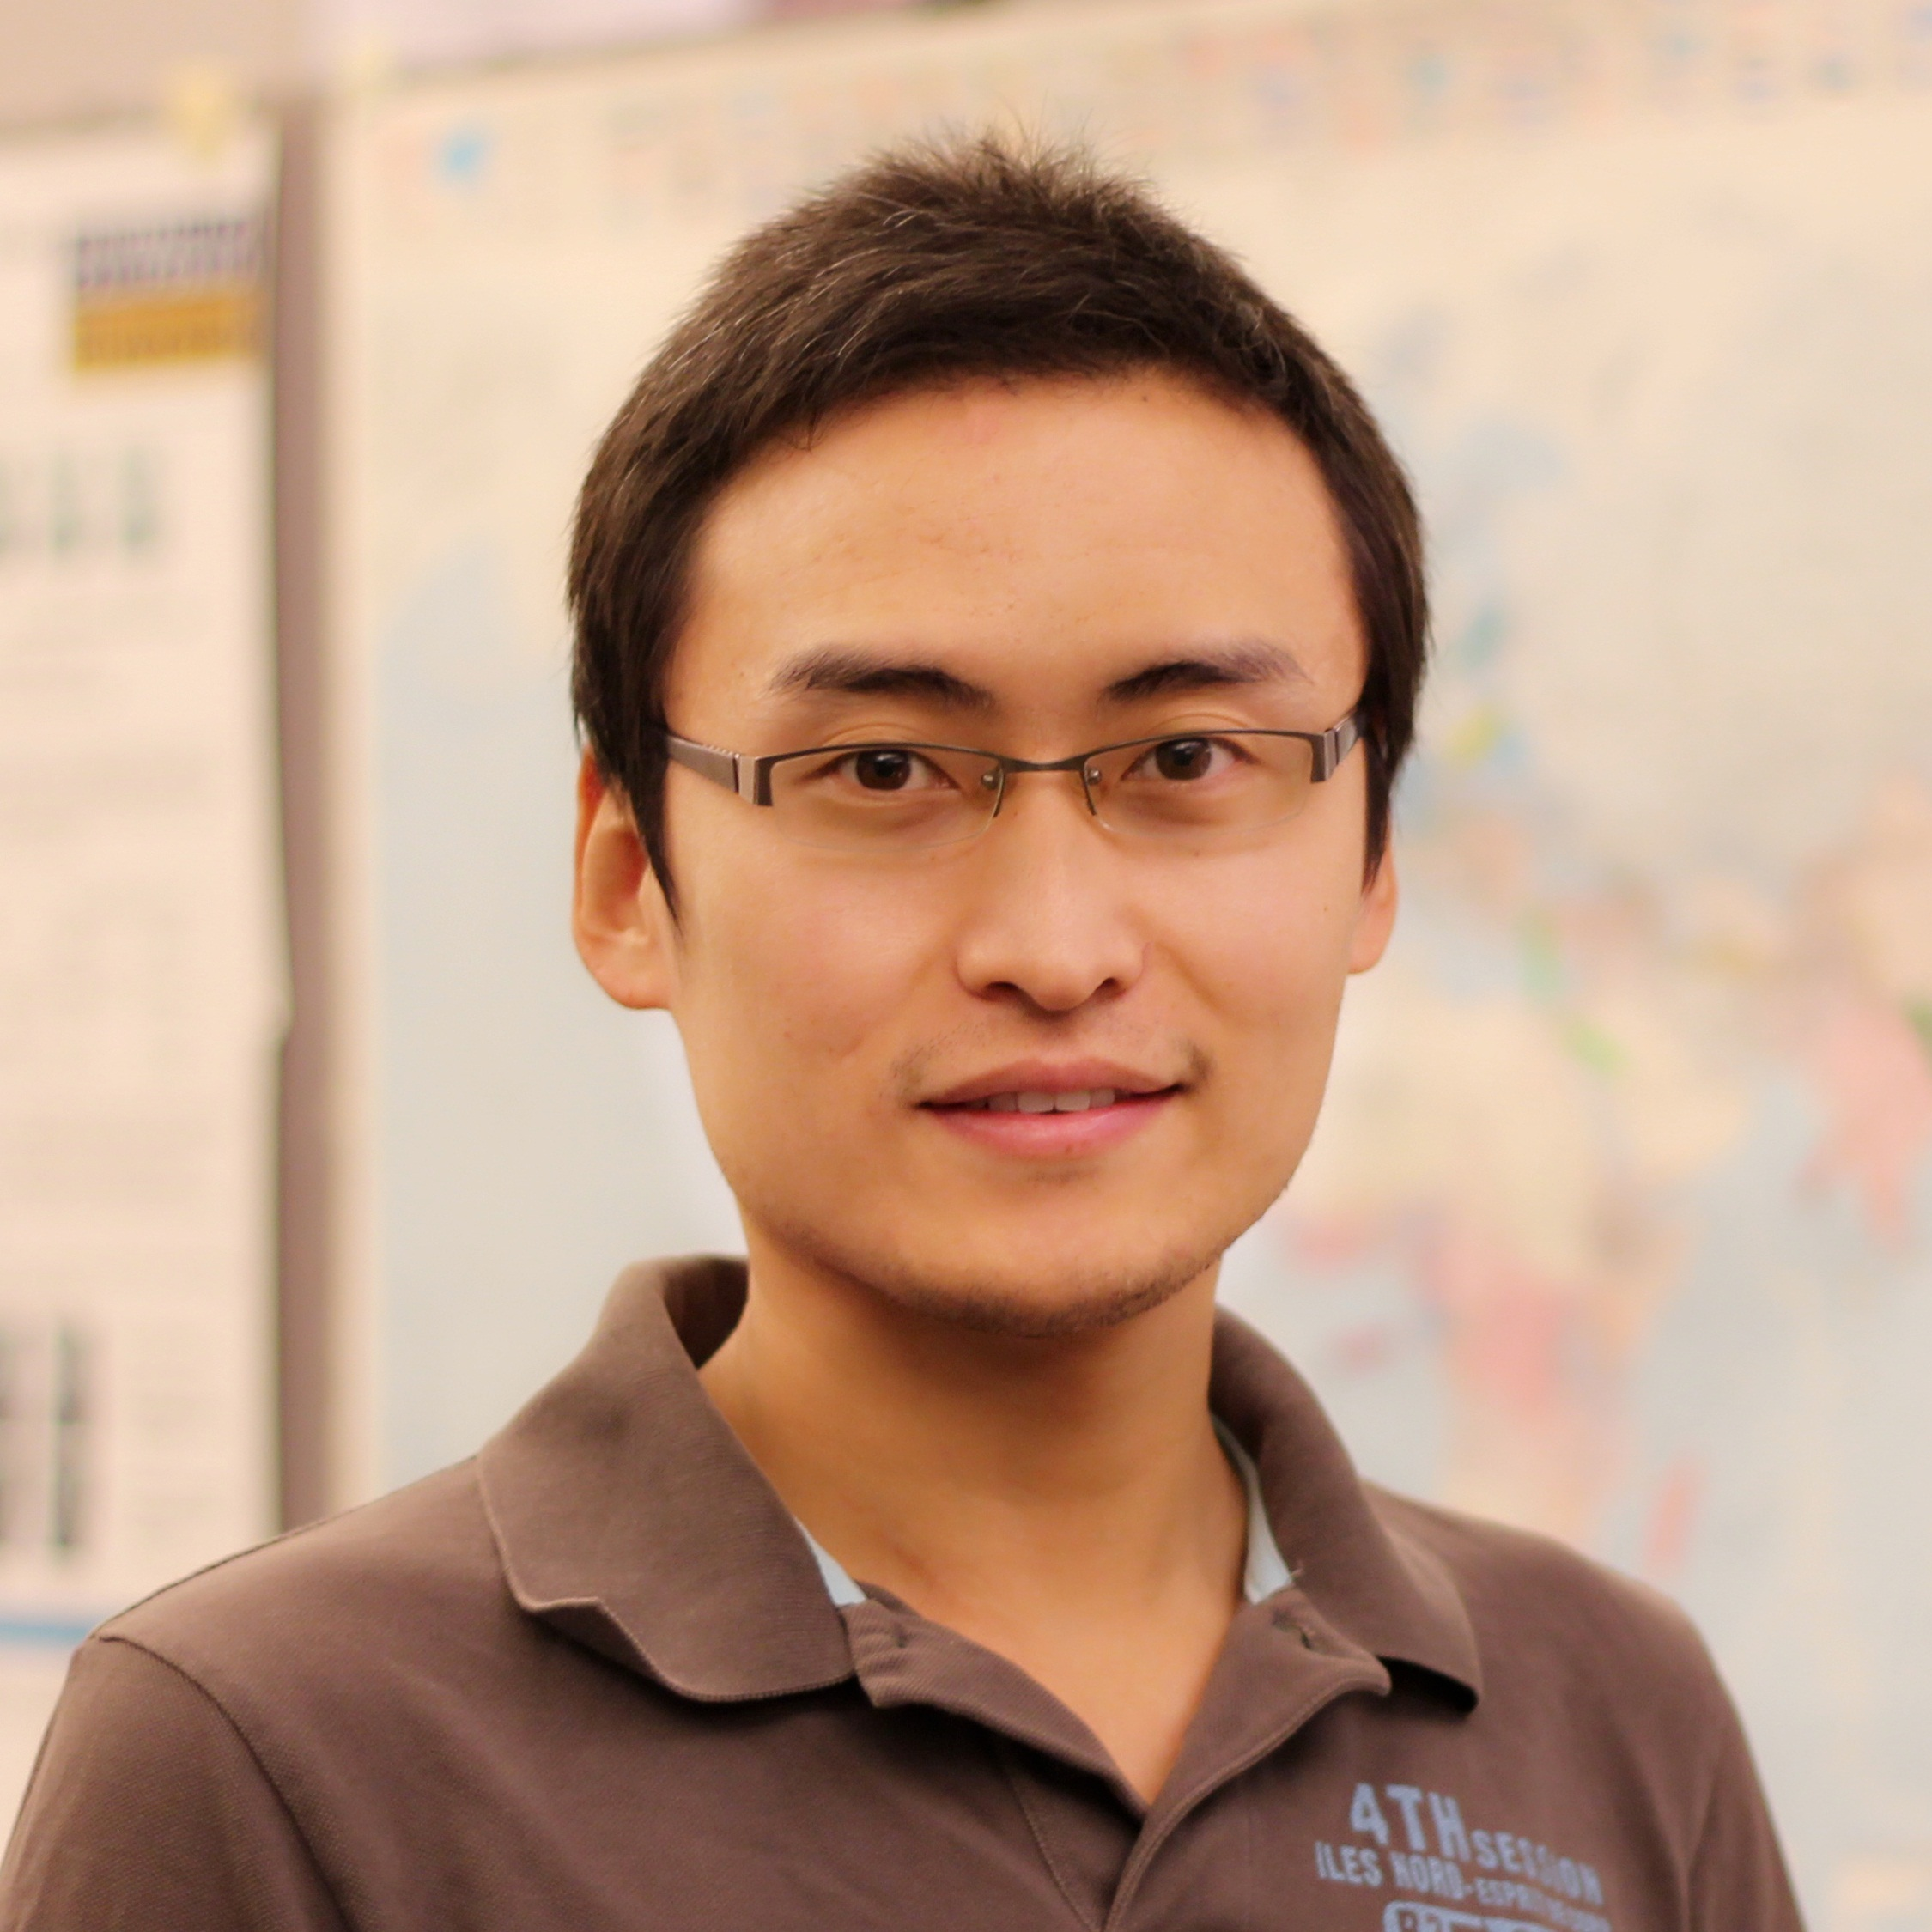
\includegraphics[width=1in,height=1.25in,clip,keepaspectratio]{pic/Lean.jpg}}]{Le An} received the B.Eng. degree in telecommunications engineering from Zhejiang University in China in 2006, the MSc degree in electrical engineering from Eindhoven University of Technology in Netherlands in 2008, and the PhD degree in electrical engineering from University of California, Riverside in USA in 2014. He is currently a postdoctoral research associate at University of North Carolina at Chapel Hill, USA.  
His research interests include image processing, computer vision, pattern recognition, and machine learning. He received the best paper award from the 2013 IEEE International Conference on Advanced Video and Signal-Based Surveillance (AVSS).
\end{IEEEbiography}

\begin{IEEEbiography}[{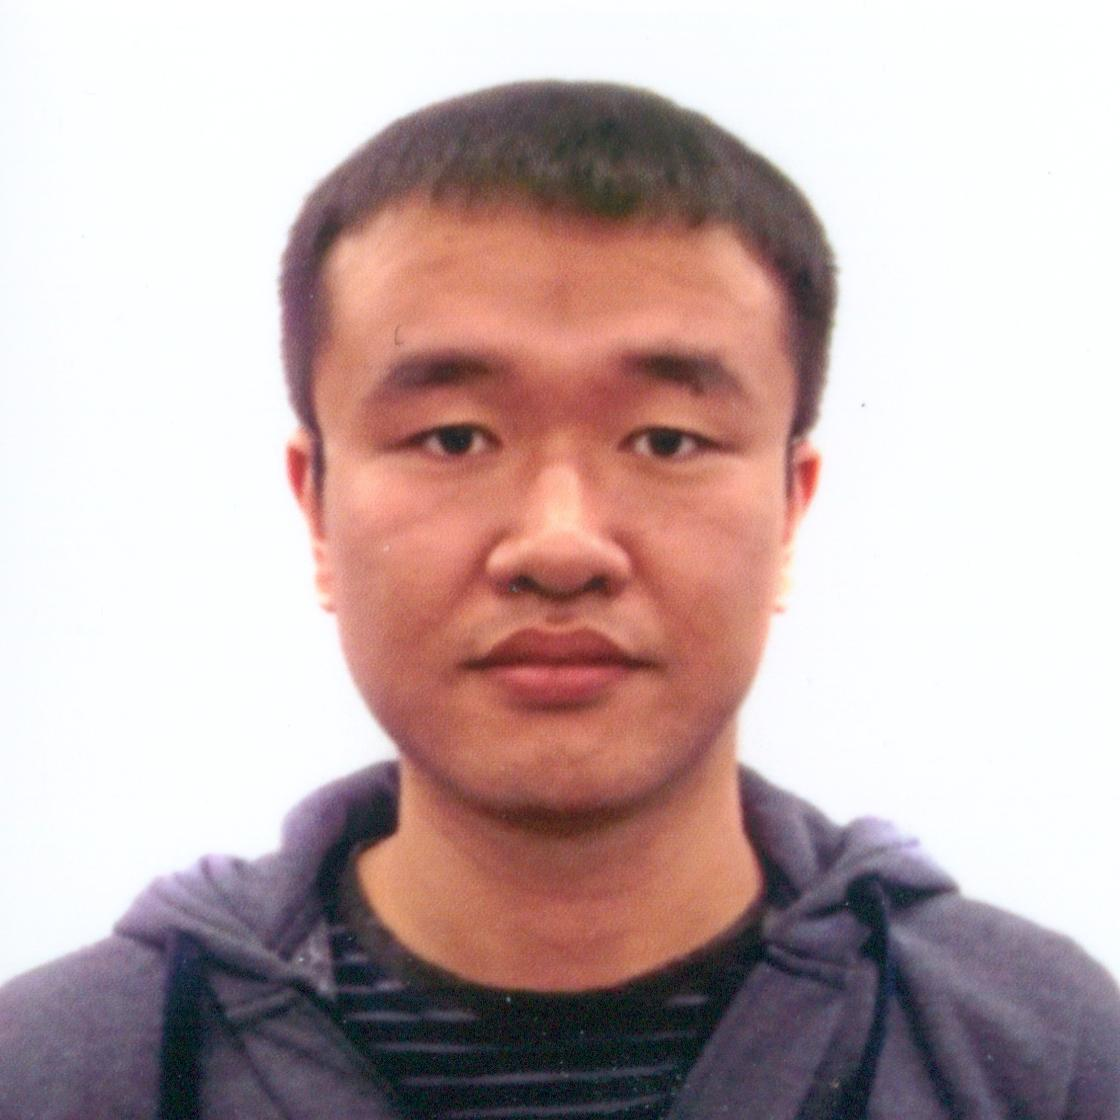
\includegraphics[width=1in,height=1.25in,clip,keepaspectratio]{pic/mingyang.jpg}}]{Mingyang Li} received the B.Eng. degree in Automation Engineering from University of Electronic Science and Technology of China, Chengdu, China, in 2009 and the M.S. degree in
Electrical Engineering from University of California, Riverside, in 2012.
He is currently a Ph.D. student in Electrical Engineering at the University of California, Riverside. His research interest lies primarily in the areas of robotics and computer vision. In particular, his research focuses sensor fusion, vision-aided inertial navigation, and multiple-view geometry in computer vision. 
\end{IEEEbiography}


\begin{IEEEbiography}[{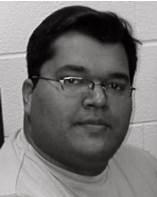
\includegraphics[width=1in,height=1.25in,clip,keepaspectratio]{pic/ninad}}]{Ninad Thakoor} 
(S'04-M'10) received the BE degree in electronics and telecommunication engineering from the University of Mumbai, India, in 2001, and the MS and PhD degrees in electrical engineering from the University of Texas at Arlington, in 2004 and 2009, respectively. He is with Center for Research in Intelligent System at University of California at Riverside as a postdoctoral researcher.

His current research interests include vehicle recognition, stereo disparity segmentation, and structure-and-motion segmentation.
\end{IEEEbiography}



\begin{IEEEbiography}[{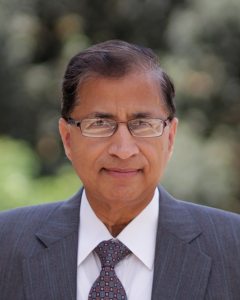
\includegraphics[width=1in,height=1.25in,clip,keepaspectratio]{pic/bhanu}}]{Bir Bhanu}
(S'72-M'82-SM'87-F'95) received the S.M. and E.E. degrees in Electrical Engineering and Computer Science from the Massachusetts Institute of Technology, Cambridge, MA, the Ph.D. degree in Electrical Engineering, from the Image Processing Institute at University of Southern California and the M.B.A. degree from the University of California, Irvine. He is the Distinguished Professor of Electrical Engineering and Cooperative Professor of Computer Science and Engineering, Mechanical Engineering and Bioengineering, and the Director of the Center for Research in Intelligent Systems (CRIS) and the Visualization and Intelligent Systems Laboratory (VISLab) at the University of California, Riverside (UCR). In addition, he serves as the director of NSF IGERT on Video Bioinformatics at UCR. Dr. Bhanu has been the Principal Investigator of various programs for NSF, DARPA, NASA, AFOSR, ONR, ARO, and other agencies and industries in the areas of video networks, video understanding, video bioinformatics, learning and vision, image understanding, pattern recognition, target recognition, biometrics, autonomous navigation, image databases, and machine-vision applications. He has published seven coauthored and three edited books. He is the holder of 18 (5 pending) patents. He has published more than 450 reviewed technical publications, including over 120 journal papers and 45 book chapters. His current research interests are Computer Vision, Pattern Recognition and Data Mining, Machine Learning, Artificial Intelligence, Image Processing, Image and Video Database, Graphics and Visualization, Robotics, Human-Computer Interactions, Biological, Medical, Military and Intelligence applications. He is Fellow of IEEE, AAAS, IAPR, and SPIE.
\end{IEEEbiography}


% if you will not have a photo at all:


% You can push biographies down or up by placing
% a \vfill before or after them. The appropriate
% use of \vfill depends on what kind of text is
% on the last page and whether or not the columns
% are being equalized.

%\vfill

% Can be used to pull up biographies so that the bottom of the last one
% is flush with the other column.
%\enlargethispage{-5in}



% that's all folks
\end{document}
